%%%%%%%%%%%%%%
%% Run LaTeX on this file several times to get Table of Contents,
%% cross-references, and citations.

%% If you have font problems, you may edit the w-bookps.sty file
%% to customize the font names to match those on your system.

%% w-bksamp.tex. Current Version: Feb 16, 2012
%%%%%%%%%%%%%%%%%%%%%%%%%%%%%%%%%%%%%%%%%%%%%%%%%%%%%%%%%%%%%%%%
%
%  Sample file for
%  Wiley Book Style, Design No.: SD 001B, 7x10
%  Wiley Book Style, Design No.: SD 004B, 6x9
%
%
%  Prepared by Amy Hendrickson, TeXnology Inc.
%  http://www.texnology.com
%%%%%%%%%%%%%%%%%%%%%%%%%%%%%%%%%%%%%%%%%%%%%%%%%%%%%%%%%%%%%%%%

%%%%%%%%%%%%%
% 7x10
%\documentclass{wileySev}

% 6x9
\documentclass{wileySix}

\usepackage{graphicx}
\usepackage{listings}
\usepackage{float}
\usepackage{color}

\definecolor{codegreen}{rgb}{0,0.6,0}
\definecolor{codegray}{rgb}{0.5,0.5,0.5}
\definecolor{codepurple}{rgb}{0.58,0,0.82}
\definecolor{backcolour}{rgb}{0.95,0.95,0.92}

\lstdefinestyle{mystyle}{
    backgroundcolor=\color{backcolour},
    commentstyle=\color{codegreen},
    keywordstyle=\color{magenta},
    numberstyle=\tiny\color{codegray},
    stringstyle=\color{codepurple},
    basicstyle=\footnotesize,
    breakatwhitespace=false,
    breaklines=true,
    captionpos=b,
    keepspaces=true,
    numbers=left,
    numbersep=5pt,
    showspaces=false,
    showstringspaces=false,
    showtabs=false,
    tabsize=2,
    language=sh
}

\lstset{style=mystyle}

%%%%%%%
%% for times math: However, this package disables bold math (!)
%% \mathbf{x} will still work, but you will not have bold math
%% in section heads or chapter titles. If you don't use math
%% in those environments, mathptmx might be a good choice.

% \usepackage{mathptmx}

% For PostScript text
\usepackage{w-bookps}

%%%%%%%%%%%%%%%%%%%%%%%%%%%%%%%%%%%%%%%%%%%%%%%%%%%%%%%%%%%%%%%%
%% Other packages you might want to use:

% for chapter bibliography made with BibTeX
% \usepackage{chapterbib}

% for multiple indices
% \usepackage{multind}

% for answers to problems
% \usepackage{answers}

%%%%%%%%%%%%%%%%%%%%%%%%%%%%%%
%% Change options here if you want:
%%
%% How many levels of section head would you like numbered?
%% 0= no section numbers, 1= section, 2= subsection, 3= subsubsection
%%==>>
\setcounter{secnumdepth}{3}

%% How many levels of section head would you like to appear in the
%% Table of Contents?
%% 0= chapter titles, 1= section titles, 2= subsection titles,
%% 3= subsubsection titles.
%%==>>
\setcounter{tocdepth}{2}

%% Cropmarks? good for final page makeup
%% \docropmarks

%%%%%%%%%%%%%%%%%%%%%%%%%%%%%%
%
% DRAFT
%
% Uncomment to get double spacing between lines, current date and time
% printed at bottom of page.
% \draft
% (If you want to keep tables from becoming double spaced also uncomment
% this):
% \renewcommand{\arraystretch}{0.6}
%%%%%%%%%%%%%%%%%%%%%%%%%%%%%%

%%%%%%% Demo of section head containing sample macro:
%% To get a macro to expand correctly in a section head, with upper and
%% lower case math, put the definition and set the box
%% before \begin{document}, so that when it appears in the
%% table of contents it will also work:

\newcommand{\VT}[1]{\ensuremath{{V_{T#1}}}}

%% use a box to expand the macro before we put it into the section head:

\newbox\sectsavebox
\setbox\sectsavebox=\hbox{\boldmath\VT{xyz}}

%%%%%%%%%%%%%%%%% End Demo


\begin{document}


\booktitle{Cerdas Menguasai Python}
\subtitle{Dalam 24 Jam}

\authors{Rolly M. Awangga\\
\affil{Informatics Research Center}
%Floyd J. Fowler, Jr.\\
%\affil{University of New Mexico}
}

\offprintinfo{Cerdas Menguasai Python, First Edition}{Rolly M. Awangga}

%% Can use \\ if title, and edition are too wide, ie,
%% \offprintinfo{Survey Methodology,\\ Second Edition}{Robert M. Groves}

%%%%%%%%%%%%%%%%%%%%%%%%%%%%%%
%%
\halftitlepage

%\titlepage


\begin{copyrightpage}{2019}
%Survey Methodology / Robert M. Groves . . . [et al.].
%\       p. cm.---(Wiley series in survey methodology)
%\    ``Wiley-Interscience."
%\    Includes bibliographical references and index.
%\    ISBN 0-471-48348-6 (pbk.)
%\    1. Surveys---Methodology.  2. Social 
%\  sciences---Research---Statistical methods.  I. Groves, Robert M.  II. %
%Series.\\
%
%HA31.2.S873 2007
%001.4'33---dc22                                             2004044064
\end{copyrightpage}

\dedication{`Jika Kamu tidak dapat menahan lelahnya belajar,
Maka kamu harus sanggup menahan perihnya Kebodohan.'
~Imam Syafi'i~}

\begin{contributors}
\name{Rolly Maulana Awangga,} Informatics Research Center., Politeknik Pos Indonesia, Bandung,
Indonesia



\end{contributors}

\contentsinbrief
\tableofcontents
\listoffigures
\listoftables
\lstlistoflistings


\begin{foreword}
Sepatah kata dari Kaprodi, Kabag Kemahasiswaan dan Mahasiswa
\end{foreword}

\begin{preface}
Buku ini diciptakan bagi yang awam dengan flask sekalipun.

\prefaceauthor{R. M. Awangga}
\where{Bandung, Jawa Barat\\
Februari, 2019}
\end{preface}


\begin{acknowledgments}
Terima kasih atas semua masukan dari para mahasiswa agar bisa membuat buku ini 
lebih baik dan lebih mudah dimengerti.

Terima kasih ini juga ditujukan khusus untuk team IRC yang 
telah fokus untuk belajar dan memahami bagaimana buku ini mendampingi proses 
Intership.
\authorinitials{R. M. A.}
\end{acknowledgments}

\begin{acronyms}
\acro{ACGIH}{American Conference of Governmental Industrial Hygienists}
\acro{AEC}{Atomic Energy Commission}
\acro{OSHA}{Occupational Health and Safety Commission}
\acro{SAMA}{Scientific Apparatus Makers Association}
\end{acronyms}

\begin{glossary}
\term{git}Merupakan manajemen sumber kode yang dibuat oleh linus torvald.

\term{bash}Merupakan bahasa sistem operasi berbasiskan *NIX.

\term{linux}Sistem operasi berbasis sumber kode terbuka yang dibuat oleh Linus Torvald
\end{glossary}

\begin{symbols}
\term{A}Amplitude

\term{\hbox{\&}}Propositional logic symbol 

\term{a}Filter Coefficient

\bigskip

\term{\mathcal{B}}Number of Beats
\end{symbols}

\begin{introduction}

%% optional, but if you want to list author:

\introauthor{Rolly Maulana Awangga, S.T., M.T.}
{Informatics Research Center\\
Bandung, Jawa Barat, Indonesia}

Pada era disruptif  \index{disruptif}\index{disruptif!modern} 
saat ini. git merupakan sebuah kebutuhan dalam sebuah organisasi pengembangan perangkat lunak.
Buku ini diharapkan bisa menjadi penghantar para programmer, analis, IT Operation dan Project Manajer.
Dalam melakukan implementasi git pada diri dan organisasinya.

Rumusnya cuman sebagai contoh aja biar keren\cite{awangga2018sampeu}.

\begin{equation}
ABC {\cal DEF} \alpha\beta\Gamma\Delta\sum^{abc}_{def}
\end{equation}

\end{introduction}

%%%%%%%%%%%%%%%%%%Isi Buku_
%TEORI
%\chapter{Judul Bagian Pertama}
%\section{Arjun Yuda Firwanda}
\subsection{Soal 1}
Isi jawaban soal ke-1

Kalau mau dibikin paragrap \textbf{cukup enter aja}, tidak usah pakai \verb|par| dsb

%\subsection{Soal 2}
%Isi jawaban soal ke-2

%\subsection{Soal 3}
%Isi jawaban soal ke-3

\section{Dwi Yulianingsih}
\subsection{Soal 1}
Isi jawaban soal ke-1

Kalau mau dibikin paragrap \textbf{cukup enter aja}, tidak usah pakai \verb|par| dsb

%\subsection{Soal 2}
%Isi jawaban soal ke-2

%\subsection{Soal 3}
%Isi jawaban soal ke-3

\section{Harun Ar-Rasyid}
\subsection{Soal 1}
Isi jawaban soal ke-1

Kalau mau dibikin paragrap \textbf{cukup enter aja}, tidak usah pakai \verb|par| dsb

%\subsection{Soal 2}
%Isi jawaban soal ke-2

%\subsection{Soal 3}
%Isi jawaban soal ke-3

\section{Sri Rahayu}
\subsection{Soal 1}
Isi jawaban soal ke-1

Kalau mau dibikin paragrap \textbf{cukup enter aja}, tidak usah pakai \verb|par| dsb

%\subsection{Soal 2}
%Isi jawaban soal ke-2

%\subsection{Soal 3}
%Isi jawaban soal ke-3

\section{Doli Jonviter}
\subsection{Soal 1}
Isi jawaban soal ke-1

Kalau mau dibikin paragrap \textbf{cukup enter aja}, tidak usah pakai \verb|par| dsb

%\subsection{Soal 2}
%Isi jawaban soal ke-2

%\subsection{Soal 3}
%Isi jawaban soal ke-3

\section{Rahmatul Ridha}
\subsection{Sejarah Python}
Bahasa pemrograman Python adalah bahasa yang dibuat oleh seorang keturunan Belanda yaitu Guido van Rossum. Sampai saat ini Python masih dikembangkan oleh \textit{Python Software Foundation}. Awalnya, pembuatan bahasa pemrograman ini adalah untuk membuat skrip bahasa tingkat tinggi pada sebuah sistem operasi yang terdistribusi Amoeba. Python telah digunakan oleh beberapa pengembang dan bahkan digunakan oleh beberapa perusahaan untuk pembuatan perangkat lunak komersial. Pemrograman bahasa python ini adalah pemrogram gratis atau \textit{freeware}, sehingga dapat dikembangkan, dan tidak ada batasan dalam penyalinannya dan mendistribusikan.

Saat ini pengembangan Python terus dilakukan oleh sekumpulan pemrogram yang dikoordinir Guido dan Python Software Foundation. Python Software Foundation adalah sebuah organisasi non-profit yang dibentuk sebagai pemegang hak cipta intelektual Python sejak versi 2.1 dan dengan demikian mencegah Python dimiliki oleh perusahaan komersial. Saat ini distribusi Python sudah mencapai versi 2.7.14 dan versi 3.6.3.


\section{Tomy Prawoto}
\subsection{Soal 1}
Isi jawaban soal ke-1

Kalau mau dibikin paragrap \textbf{cukup enter aja}, tidak usah pakai \verb|par| dsb

%\subsection{Soal 2}
%Isi jawaban soal ke-2

%\subsection{Soal 3}
%Isi jawaban soal ke-3

%PRAKTEK
%\chapter{Judul Bagian Pertama}
%\section{Arjun Yuda Firwanda}
\subsection{Soal 1}
Isi jawaban soal ke-1

Kalau mau dibikin paragrap \textbf{cukup enter aja}, tidak usah pakai \verb|par| dsb

%\subsection{Soal 2}
%Isi jawaban soal ke-2

%\subsection{Soal 3}
%Isi jawaban soal ke-3

\section{Dwi Yulianingsih}
\subsection{Soal 1}
Isi jawaban soal ke-1

Kalau mau dibikin paragrap \textbf{cukup enter aja}, tidak usah pakai \verb|par| dsb

%\subsection{Soal 2}
%Isi jawaban soal ke-2

%\subsection{Soal 3}
%Isi jawaban soal ke-3

\section{Harun Ar-Rasyid}
\subsection{Soal 1}
Isi jawaban soal ke-1

Kalau mau dibikin paragrap \textbf{cukup enter aja}, tidak usah pakai \verb|par| dsb

%\subsection{Soal 2}
%Isi jawaban soal ke-2

%\subsection{Soal 3}
%Isi jawaban soal ke-3

\section{Sri Rahayu}
\subsection{Soal 1}
Isi jawaban soal ke-1

Kalau mau dibikin paragrap \textbf{cukup enter aja}, tidak usah pakai \verb|par| dsb

%\subsection{Soal 2}
%Isi jawaban soal ke-2

%\subsection{Soal 3}
%Isi jawaban soal ke-3

\section{Doli Jonviter}
\subsection{Soal 1}
Isi jawaban soal ke-1

Kalau mau dibikin paragrap \textbf{cukup enter aja}, tidak usah pakai \verb|par| dsb

%\subsection{Soal 2}
%Isi jawaban soal ke-2

%\subsection{Soal 3}
%Isi jawaban soal ke-3

\section{Rahmatul Ridha}
\subsection{Soal 1}
\subsection{Instalasi Anaconda}
\begin{itemize}
\item Instalasi Anaconda
Berikut adalah langkah-langkah cara menginstal Anaconda di Windows:
\begin{enumerate}
\item Download installer anaconda terbaru, seperti pada gambar \ref{downloadanaconda}. Kalian dapat memilih versi 2 atau 3, dengan versi Anaconda berapa.
\begin{figure}[ht] \centerline{\includegraphics[width=0.70\textwidth]{figures/1/1144124/DownloadAnaconda.JPG}}
	\caption{Download Anaconda}
	\label{downloadanaconda}
\end{figure}
	
\item Setelah selesai mendownload, klik 2 kali pada installer Anaconda.
\item Kemudian akan tampil seperti gambar \ref{gambar1}, lalu klik next.
\begin{figure}[ht]
	\centerline{\includegraphics[width=0.70\textwidth]{figures/1/1144124/a.JPG}}
	\caption{Proses 1 }
	\label{gambar1}
\end{figure}

\item Setelah itu read lisensi dan klik `I Agree' seperti pada gambar \ref{gambar2}.
\begin{figure}[ht]
	\centerline{\includegraphics[width=0.70\textwidth]{figures/1/1144124/b.JPG}}
	\caption{proses 2 }
	\label{gambar2}
\end{figure}

\item Selanjutnya ada pilihan untuk menginstallnya, yaitu `just me' atau `all users'. Lalu klik next seperti pada gambar \ref{gambar3}.
\begin{figure}[ht]
	\centerline{\includegraphics[width=0.70\textwidth]{figures/1/1144124/c.JPG}}
	\caption{Proses 3 }
	\label{gambar3}
\end{figure}

\item Kemudian pilih okasi yang diinginkan, lalu klik next seperti pada gambar \ref{gambar4}.
\begin{figure}[ht]
	\centerline{\includegraphics[width=0.70\textwidth]{figures/1/1144124/d.JPG}}
	\caption{Proses 4 }
	\label{gambar4}
\end{figure}

\item Pilih ‘add anaconda to PATH’ atau tidak. Disini kalian memilih apakah akan mendaftarkan Anaconda sebagai default Python 3.7. kacuali kalian berencana menginstal dan menjalankan beberapa versi Anaconda, atau beberapa versi Python, biarkan default dan biarkan kotaknya dicentang. Kemudian klik tombol Install. Jika kalian ingin melihat packages Anaconda yang sedang dipasang, klik Show Details seperti pada gambar \ref{gambar5}.
\begin{figure}[ht]
	\centerline{\includegraphics[width=0.70\textwidth]{figures/1/1144124/e.JPG}}
	\caption{Proses 5 }
	\label{gambar5}
\end{figure}

\item Jika instalasi selesai, kemudian klik next seperti pada gambar \ref{gambar6}.
\begin{figure}[ht]
	\centerline{\includegraphics[width=0.70\textwidth]{figures/1/1144124/f.JPG}}
	\caption{Proses 6 }
	\label{gambar6}
\end{figure}

\item Jika packages telah selesai diinstall, maka aka nada perintah untuk menginstall VS Code, lalu klik tombol Install Microsoft VS Code seperti pada gambar \ref{gambar7}.
\begin{figure}[ht]
	\centerline{\includegraphics[width=0.70\textwidth]{figures/1/1144124/g.JPG}}
	\caption{Proses 7}
	\label{gambar7}
\end{figure}

\item Setelah instalasi selesai, maka akan terlihat kotal dialog `Thanks for Installing Anaconda3'. Lalu klik Finish seperti pada gambar \ref{gambar8}.
\begin{figure}[ht]
	\centerline{\includegraphics[width=0.70\textwidth]{figures/1/1144124/h.JPG}}
	\caption{Proses 8}
	\label{gambar8}
\end{figure}
	    \end{enumerate}
\end{itemize}

\section{Tomy Prawoto}
\subsection{Soal 1}
\subsection{Instalasi Anaconda}
\begin{itemize}
\item Instalasi Anaconda
Berikut adalah langkah-langkah cara menginstal Anaconda di Windows:
\begin{enumerate}
\item Download installer anaconda terbaru, seperti pada gambar \ref{downloadanaconda}. Kalian dapat memilih versi 2 atau 3, dengan versi Anaconda berapa.
\begin{figure}[ht]
	\centerline{\includegraphics[width=0.70\textwidth]{figures/1/1154121/DownloadAnaconda.JPG}}
	\caption{Download Anaconda}
	\label{downloadanaconda}
\end{figure}	
\item Setelah selesai mendownload, klik 2 kali pada installer Anaconda.
\item Kemudian akan tampil seperti gambar \ref{gambar1}, lalu klik next.
\begin{figure}[ht]
	\centerline{\includegraphics[width=0.70\textwidth]{figures/1/1154121/a.JPG}}
	\caption{Proses 1 }
	\label{gambar1}
\end{figure}
\item Setelah itu read lisensi dan klik “I Agree”.
\begin{figure}[ht]
	\centerline{\includegraphics[width=0.70\textwidth]{figures/1/1154121/b.JPG}}
	\caption{proses 2 }
	\label{gambar2 }
\end{figure}

\item Selanjutnya ada pilihan untuk menginstallnya, yaitu “just me” atau “all users”. Lalu klik next.
\begin{figure}[ht]
	\centerline{\includegraphics[width=0.70\textwidth]{figures/1/1154121/c.JPG}}
	\caption{Proses 3 }
	\label{gambar3}
\end{figure}

\item Kemudian pilih okasi yang diinginkan, lalu klik next.
\begin{figure}[ht]
	\centerline{\includegraphics[width=0.70\textwidth]{figures/1/1154121/d.JPG}}
	\caption{Proses 4 }
	\label{gambar4 }
\end{figure}

\item Pilih ‘add anaconda to PATH’ atau tidak. Disini kalian memilih apakah akan mendaftarkan Anaconda sebagai default Python 3.7. kacuali kalian berencana menginstal dan menjalankan beberapa versi Anaconda, atau beberapa versi Python, biarkan default dan biarkan kotaknya dicentang. Kemudian klik tombol Install. Jika kalian ingin melihat packages Anaconda yang sedang dipasang, klik Show Details.
\begin{figure}[ht]
	\centerline{\includegraphics[width=0.70\textwidth]{figures/1/1154121/e.JPG}}
	\caption{Proses 5 }
	\label{gambar5 }
\end{figure}

\item Jika instalasi selesai, kemudian klik next.
\begin{figure}[ht]
	\centerline{\includegraphics[width=0.70\textwidth]{figures/1/1154121/f.JPG}}
	\caption{Proses 6 }
	\label{gambar6 }
\end{figure}

\item Jika packages telah selesai diinstall, maka aka nada perintah untuk menginstall VS Code, lalu klik tombol Install Microsoft VS Code.
\begin{figure}[ht]
	\centerline{\includegraphics[width=0.70\textwidth]{figures/1/1154121/g.JPG}}
	\caption{Proses 7}
	\label{gambar7 }
\end{figure}

\item Setelah instalasi selesai, maka akan terlihat kotal dialog “Thanks for Installing Anaconda3”. Lalu klik Finish.
\begin{figure}[ht]
	\centerline{\includegraphics[width=0.70\textwidth]{figures/1/1154121/h.JPG}}
	\caption{Proses 8}
	\label{gambar8 }
\end{figure}
	    \end{enumerate}
\end{itemize} 


%TEORI
%\chapter{Judul Bagian Pertama}
%\section{Arjun Yuda Firwanda}
\subsection{Soal 1}
Isi jawaban soal ke-1

Kalau mau dibikin paragrap \textbf{cukup enter aja}, tidak usah pakai \verb|par| dsb

%\subsection{Soal 2}
%Isi jawaban soal ke-2

%\subsection{Soal 3}
%Isi jawaban soal ke-3

\section{Dwi Yulianingsih}
\subsection{Soal 1}
Isi jawaban soal ke-1

Kalau mau dibikin paragrap \textbf{cukup enter aja}, tidak usah pakai \verb|par| dsb

%\subsection{Soal 2}
%Isi jawaban soal ke-2

%\subsection{Soal 3}
%Isi jawaban soal ke-3

\section{Harun Ar-Rasyid}
\subsection{Soal 1}
Isi jawaban soal ke-1

Kalau mau dibikin paragrap \textbf{cukup enter aja}, tidak usah pakai \verb|par| dsb

%\subsection{Soal 2}
%Isi jawaban soal ke-2

%\subsection{Soal 3}
%Isi jawaban soal ke-3

\section{Sri Rahayu}
\subsection{Soal 1}
Isi jawaban soal ke-1

Kalau mau dibikin paragrap \textbf{cukup enter aja}, tidak usah pakai \verb|par| dsb

%\subsection{Soal 2}
%Isi jawaban soal ke-2

%\subsection{Soal 3}
%Isi jawaban soal ke-3

\section{Doli Jonviter}
\subsection{Soal 1}
Isi jawaban soal ke-1

Kalau mau dibikin paragrap \textbf{cukup enter aja}, tidak usah pakai \verb|par| dsb

%\subsection{Soal 2}
%Isi jawaban soal ke-2

%\subsection{Soal 3}
%Isi jawaban soal ke-3

\section{Rahmatul Ridha}
\subsection{Teori}
\begin{enumerate}
\item jenis-jenis variable phyton dan cara pemakaiannya. Variable merupakan tempat untuk menyimpan data, Isi dari variabel itu dapat berubah atau mutable sesuai dengan operasi yang diinginkan. Saat program dieksekusi maka variabellah yang bertugas menyimpan data. Dimana didalam phyton terdapat beberapa variable diantaranya number, boolean,string. Dalam membuat variabel Pythoncaranya adalah sebagai berikut
    \lstinputlisting[firstline=8,lastline=46]{src/2/1144124/1144124_Teori.py}

\item operator dasar aritmatika. Dimana terdapat penjumlahan,pengurangan,pembagian,perkalian,perpangkatan,pembulatan nominal
    \lstinputlisting[firstline=47,lastline=75]{src/2/1144124/1144124_Teori.py}

\item Perulangan. Dalam phyton terdapat perulangan while dan for :
    \lstinputlisting[firstline=76,lastline=87]{src/2/1144124/1144124_Teori.py}

\item Dimana terdapat sintak untuk memilih kondisi didalam kondisi. Untuk memilih keputusan menggunakan (kondisi if) dimana digunakan untuk mengantisipasi kondisi yang terjadi saat jalannya suatu program dan menentukan tindakan apa yang akan dilakukan sesuai dengan kondisi.
    \lstinputlisting[firstline=88,lastline=112]{src/2/1144124/1144124_Teori.py}

\item Jenis-jenis sintak error pada phyton.

Syntax errors Jika dalam program terdapat kesalahan sintaks maka proses akan berhenti dan menampilkan pesan kesalahan.
Runtime errors, disebut begitu karenakesalahan tidak akan muncul sampai Anda menjalankan program tersebut.Kesalahan ini juga dikenal dengan exceptions atau pengecualian karena biasanya mengindikasikan sesuatu pengecualian yang buruk telah terjadi.

Type eror merupakan eror yang terjadi saat dilakukan eksekusi pada suatu operasi dengan type object yang tidak sesuai.
ZeroDivision eror merupakan eror yang terjadi saat eksekusi program menghasilkan perhitungan matematika dengan angka 0

\item Try except
cara memakai try except adalah sebagai berikut
    \lstinputlisting[firstline=8,lastline=17]{src/2/1144124/1144124_Teori.py}
    \end{enumerate}

\section{Tomy Prawoto}
\subsection{Soal 1}
Isi jawaban soal ke-1

Kalau mau dibikin paragrap \textbf{cukup enter aja}, tidak usah pakai \verb|par| dsb

%\subsection{Soal 2}
%Isi jawaban soal ke-2

%\subsection{Soal 3}
%Isi jawaban soal ke-3

%PRAKTEK
%\chapter{Judul Bagian Pertama}
%\section{Arjun Yuda Firwanda}
\subsection{Soal 1}
Isi jawaban soal ke-1

Kalau mau dibikin paragrap \textbf{cukup enter aja}, tidak usah pakai \verb|par| dsb

%\subsection{Soal 2}
%Isi jawaban soal ke-2

%\subsection{Soal 3}
%Isi jawaban soal ke-3

\section{Dwi Yulianingsih}
\subsection{Soal 1}
Isi jawaban soal ke-1

Kalau mau dibikin paragrap \textbf{cukup enter aja}, tidak usah pakai \verb|par| dsb

%\subsection{Soal 2}
%Isi jawaban soal ke-2

%\subsection{Soal 3}
%Isi jawaban soal ke-3

\section{Harun Ar-Rasyid}
\subsection{Soal 1}
Isi jawaban soal ke-1

Kalau mau dibikin paragrap \textbf{cukup enter aja}, tidak usah pakai \verb|par| dsb

%\subsection{Soal 2}
%Isi jawaban soal ke-2

%\subsection{Soal 3}
%Isi jawaban soal ke-3

\section{Sri Rahayu}
\subsection{Soal 1}
Isi jawaban soal ke-1

Kalau mau dibikin paragrap \textbf{cukup enter aja}, tidak usah pakai \verb|par| dsb

%\subsection{Soal 2}
%Isi jawaban soal ke-2

%\subsection{Soal 3}
%Isi jawaban soal ke-3

\section{Doli Jonviter}
\subsection{Soal 1}
Isi jawaban soal ke-1

Kalau mau dibikin paragrap \textbf{cukup enter aja}, tidak usah pakai \verb|par| dsb

%\subsection{Soal 2}
%Isi jawaban soal ke-2

%\subsection{Soal 3}
%Isi jawaban soal ke-3

\section{Rahmatul Ridha}
\subsection{praktek}
\begin{enumerate}
	\item Jawaban soal no 1
	\lstinputlisting[firstline=8,lastline=17]{src/2/1144124/1144124_Praktek.py}
	\item Jawaban soal no 2
	\lstinputlisting[firstline=18,lastline=23]{src/2/1144124/1144124_Praktek.py}
	\item Jawaban soal no 3
	\lstinputlisting[firstline=24,lastline=29]{src/2/1144124/1144124_Praktek.py}
	\item Jawaban soal no 4
	\lstinputlisting[firstline=30,lastline=32]{src/2/1144124/1144124_Praktek.py}
	\item Jawaban soal no 5
	\lstinputlisting[firstline=33,lastline=43]{src/2/1144124/1144124_Praktek.py}
	\item Jawaban soal no 6
	\lstinputlisting[firstline=44,lastline=45]{src/2/1144124/1144124_Praktek.py}
	\item Jawaban soal no 7
	\lstinputlisting[firstline=46,lastline=47]{src/2/1144124/1144124_Praktek.py}
	\item Jawaban soal no 8
	\lstinputlisting[firstline=48,lastline=55]{src/2/1144124/1144124_Praktek.py}
	\item Jawaban soal no 9
	\lstinputlisting[firstline=56,lastline=57]{src/2/1144124/1144124_Praktek.py}
	\item Jawaban soal no 10
	\lstinputlisting[firstline=58,lastline=59]{src/2/1144124/1144124_Praktek.py}
	\item Jawaban soal no 11
	\lstinputlisting[firstline=60,lastline=61]{src/2/1144124/1144124_Praktek.py}
\end{enumerate}

\subsection{Keterangan dan Penanganan eror}
\lstinputlisting[firstline=5,lastline=15]{src/2/1144124/error.py}

\section{Tomy Prawoto}
\subsection{Soal 1}
Isi jawaban soal ke-1

Kalau mau dibikin paragrap \textbf{cukup enter aja}, tidak usah pakai \verb|par| dsb

%\subsection{Soal 2}
%Isi jawaban soal ke-2

%\subsection{Soal 3}
%Isi jawaban soal ke-3


%TEORI
%\chapter{Judul Bagian Pertama}
%\section{Arjun Yuda Firwanda}
\subsection{Soal 1}
Isi jawaban soal ke-1

Kalau mau dibikin paragrap \textbf{cukup enter aja}, tidak usah pakai \verb|par| dsb

%\subsection{Soal 2}
%Isi jawaban soal ke-2

%\subsection{Soal 3}
%Isi jawaban soal ke-3

\section{Dwi Yulianingsih}
\subsection{Soal 1}
Isi jawaban soal ke-1

Kalau mau dibikin paragrap \textbf{cukup enter aja}, tidak usah pakai \verb|par| dsb

%\subsection{Soal 2}
%Isi jawaban soal ke-2

%\subsection{Soal 3}
%Isi jawaban soal ke-3

\section{Harun Ar-Rasyid}
\subsection{Soal 1}
Isi jawaban soal ke-1

Kalau mau dibikin paragrap \textbf{cukup enter aja}, tidak usah pakai \verb|par| dsb

%\subsection{Soal 2}
%Isi jawaban soal ke-2

%\subsection{Soal 3}
%Isi jawaban soal ke-3

\section{Sri Rahayu}
\subsection{Soal 1}
Isi jawaban soal ke-1

Kalau mau dibikin paragrap \textbf{cukup enter aja}, tidak usah pakai \verb|par| dsb

%\subsection{Soal 2}
%Isi jawaban soal ke-2

%\subsection{Soal 3}
%Isi jawaban soal ke-3

\section{Doli Jonviter}
\subsection{Soal 1}
Isi jawaban soal ke-1

Kalau mau dibikin paragrap \textbf{cukup enter aja}, tidak usah pakai \verb|par| dsb

%\subsection{Soal 2}
%Isi jawaban soal ke-2

%\subsection{Soal 3}
%Isi jawaban soal ke-3

\section{Rahmatul Ridha}
\subsection{Soal 1}
Isi jawaban soal ke-1

Kalau mau dibikin paragrap \textbf{cukup enter aja}, tidak usah pakai \verb|par| dsb

%\subsection{Soal 2}
%Isi jawaban soal ke-2

%\subsection{Soal 3}
%Isi jawaban soal ke-3

\section{Tomy Prawoto}
\subsection{Soal 1}
Isi jawaban soal ke-1

Kalau mau dibikin paragrap \textbf{cukup enter aja}, tidak usah pakai \verb|par| dsb

%\subsection{Soal 2}
%Isi jawaban soal ke-2

%\subsection{Soal 3}
%Isi jawaban soal ke-3

%PRAKTEK
%\chapter{Judul Bagian Pertama}
%\section{Arjun Yuda Firwanda}
\subsection{Soal 1}
Isi jawaban soal ke-1

Kalau mau dibikin paragrap \textbf{cukup enter aja}, tidak usah pakai \verb|par| dsb

%\subsection{Soal 2}
%Isi jawaban soal ke-2

%\subsection{Soal 3}
%Isi jawaban soal ke-3

\section{Dwi Yulianingsih}
\subsection{Soal 1}
Isi jawaban soal ke-1

Kalau mau dibikin paragrap \textbf{cukup enter aja}, tidak usah pakai \verb|par| dsb

%\subsection{Soal 2}
%Isi jawaban soal ke-2

%\subsection{Soal 3}
%Isi jawaban soal ke-3

\section{Harun Ar-Rasyid}
\subsection{Soal 1}
Isi jawaban soal ke-1

Kalau mau dibikin paragrap \textbf{cukup enter aja}, tidak usah pakai \verb|par| dsb

%\subsection{Soal 2}
%Isi jawaban soal ke-2

%\subsection{Soal 3}
%Isi jawaban soal ke-3

\section{Sri Rahayu}
\subsection{Soal 1}
Isi jawaban soal ke-1

Kalau mau dibikin paragrap \textbf{cukup enter aja}, tidak usah pakai \verb|par| dsb

%\subsection{Soal 2}
%Isi jawaban soal ke-2

%\subsection{Soal 3}
%Isi jawaban soal ke-3

\section{Doli Jonviter}
\subsection{Soal 1}
Isi jawaban soal ke-1

Kalau mau dibikin paragrap \textbf{cukup enter aja}, tidak usah pakai \verb|par| dsb

%\subsection{Soal 2}
%Isi jawaban soal ke-2

%\subsection{Soal 3}
%Isi jawaban soal ke-3

\section{Rahmatul Ridha}
\subsubsection{Ketrampilan Pemrograman}
\begin{enumerate}
    \item Buatlah fungsi dengan inputan variabel NPM, dan melakukan print luaran huruf yang dirangkai dari tanda bintang, pagar atau plus dari NPM kita. Tanda bintang untuk NPM mod 3=0, tanda pagar untuk NPM mod 3 =1, tanda plus untuk NPM mod3=2.
    \lstinputlisting[firstline=69, lastline=103]{src/3/1144124/1144124Chapter3.py}

    \item Buatlah fungsi dengan inputan variabel berupa NPM. kemudian dengan menggunakan perulangan mengeluarkan print output sebanyak dua dijit belakang NPM.
    \lstinputlisting[firstline=105, lastline=112]{src/3/1144124/1144124Chapter3.py}

    \item Buatlah fungsi dengan dengan input variabel string bernama NPM dan beri luaran output dengan perulangan berupa tiga karakter belakang dari NPM sebanyak penjumlahan tiga dijit tersebut.
    \lstinputlisting[firstline=114, lastline=123]{src/3/1144124/1144124Chapter3.py}

    \item Buatlah fungsi hello word dengan input variabel string bernama NPM dan beri luaran output berupa digit ketiga dari belakang dari variabel NPM menggunakan akses langsung manipulasi string pada baris ketiga dari variabel NPM.
    \lstinputlisting[firstline=125, lastline=131]{src/3/1144124/1144124Chapter3.py}

    \item buat fungsi program dengan input variabel NPM dan melakukan print nomor npm satu persatu kebawah.
    \lstinputlisting[firstline=133, lastline=138]{src/3/1144124/1144124Chapter3.py}

    \item Buatlah fungsi dengan inputan variabel NPM, didalamnya melakukan penjumlahan dari seluruh dijit NPM tersebut, wajib menggunakan perulangan dan atau kondisi.
        \lstinputlisting[firstline=140, lastline=147]{src/3/1144124/1144124Chapter3.py}

    \item Buatlah fungsi dengan inputan variabel NPM, didalamnya melakukan melakukan perkalian dari seluruh dijit NPM tersebut, wajib menggunakan perulangan dan atau kondisi.
        \lstinputlisting[firstline=149, lastline=156]{src/3/1144124/1144124Chapter3.py}

    \item Buatlah fungsi dengan inputan variabel NPM, Lakukan print NPM anda tapi hanya dijit genap saja. wajib menggunakan perulangan dan atau kondisi.
        \lstinputlisting[firstline=257, lastline=263]{src/3/1144124/1144124Chapter3.py}

    \item Buatlah fungsi dengan inputan variabel NPM, Lakukan print NPM anda tapi hanya dijit ganjil saja. wajib menggunakan perulangan dan atau kondisi.
        \lstinputlisting[firstline=158, lastline=164]{src/3/1144124/1144124Chapter3.py}

    \item Buatlah fungsi dengan inputan variabel NPM, Lakukan print NPM anda tapi hanya dikit yang termasuk bilangan prima saja. wajib menggunakan perulangan dan atau kondisi.
        \lstinputlisting[firstline=166, lastline=172]{src/3/1144124/1144124Chapter3.py}

    \item Buatlah satu library yang berisi fungsi-fungsi dari nomor diatas dengan nama file epi.py dan berikan contoh cara pemanggilannya pada file main.py.
        \lstinputlisting[firstline=8, lastline=21]{src/3/1144124/main.py}

    \item Buatlah satu library class dengan nama gile kelas3lib.py yang merupakan modifikasi dari fungsi-fungsi nomor diatas dan berikan contoh cara pemanggilannya pada file mainn.py.
        \lstinputlisting[firstline=23, lastline=38]{src/3/1144124/main.py}

\end{enumerate}

\subsubsection{Ketrampilan Penanganan Error}
Error yang di dapat dari mengerjakan tugas ini adalah type error, cara menaggulaginya dengan cara mengecheck kembali codingannya
kemudian run kembali aplikasinya. Berikut contoh Penggunaan fungsi try dan exception :
\lstinputlisting[firstline=174, lastline=188]{src/3/1144124/1144124Chapter3.py}


\section{Tomy Prawoto}
\subsection{Soal 1}
\begin{enumerate}
    \item Buatlah fungsi dengan inputan variabel NPM, dan melakukan print luaran huruf yang dirangkai dari tanda bintang, pagar atau plus dari NPM kita. Tanda bintang untuk NPM mod 3=0, tanda pagar untuk NPM mod 3 =1, tanda plus untuk NPM mod3=2.
    \lstinputlisting[firstline=69, lastline=103]{src/3/1154121/1154121Chapter3.py}

    \item Buatlah fungsi dengan inputan variabel berupa NPM. kemudian dengan menggunakan perulangan mengeluarkan print output sebanyak dua dijit belakang NPM.
    \lstinputlisting[firstline=105, lastline=112]{src/3/1154121/1154121Chapter3.py}

    \item Buatlah fungsi dengan dengan input variabel string bernama NPM dan beri luaran output dengan perulangan berupa tiga karakter belakang dari NPM sebanyak penjumlahan tiga dijit tersebut.
    \lstinputlisting[firstline=114, lastline=123]{src/3/1154121/1154121Chapter3.py}

    \item Buatlah fungsi hello word dengan input variabel string bernama NPM dan beri luaran output berupa digit ketiga dari belakang dari variabel NPM menggunakan akses langsung manipulasi string pada baris ketiga dari variabel NPM.
    \lstinputlisting[firstline=125, lastline=131]{src/3/1154121/1154121Chapter3.py}

    \item buat fungsi program dengan input variabel NPM dan melakukan print nomor npm satu persatu kebawah.
    \lstinputlisting[firstline=133, lastline=138]{src/3/1154121/1154121Chapter3.py}

    \item Buatlah fungsi dengan inputan variabel NPM, didalamnya melakukan penjumlahan dari seluruh dijit NPM tersebut, wajib menggunakan perulangan dan atau kondisi.
        \lstinputlisting[firstline=140, lastline=147]{src/3/1154121/1154121Chapter3.py}

    \item Buatlah fungsi dengan inputan variabel NPM, didalamnya melakukan melakukan perkalian dari seluruh dijit NPM tersebut, wajib menggunakan perulangan dan atau kondisi.
        \lstinputlisting[firstline=149, lastline=156]{src/3/1154121/1154121Chapter3.py}

    \item Buatlah fungsi dengan inputan variabel NPM, Lakukan print NPM anda tapi hanya dijit genap saja. wajib menggunakan perulangan dan atau kondisi.
        \lstinputlisting[firstline=257, lastline=263]{src/3/1154121/1154121Chapter3.py}

    \item Buatlah fungsi dengan inputan variabel NPM, Lakukan print NPM anda tapi hanya dijit ganjil saja. wajib menggunakan perulangan dan atau kondisi.
        \lstinputlisting[firstline=158, lastline=164]{src/3/1154121/1154121Chapter3.py}

    \item Buatlah fungsi dengan inputan variabel NPM, Lakukan print NPM anda tapi hanya dikit yang termasuk bilangan prima saja. wajib menggunakan perulangan dan atau kondisi.
        \lstinputlisting[firstline=166, lastline=172]{src/3/1154121/1154121Chapter3.py}

    \item Buatlah satu library yang berisi fungsi-fungsi dari nomor diatas dengan nama file epi.py dan berikan contoh cara pemanggilannya pada file main.py.
        \lstinputlisting[firstline=8, lastline=21]{src/3/1154121/main.py}

    \item Buatlah satu library class dengan nama gile kelas3lib.py yang merupakan modifikasi dari fungsi-fungsi nomor diatas dan berikan contoh cara pemanggilannya pada file mainn.py.
        \lstinputlisting[firstline=23, lastline=38]{src/3/1154121/main.py}

\end{enumerate}

\subsubsection{Ketrampilan Penanganan Error}
Error yang di dapat dari mengerjakan tugas ini adalah type error, cara menaggulaginya dengan cara mengecheck kembali codingannya
kemudian run kembali aplikasinya. Berikut contoh Penggunaan fungsi try dan exception :
\lstinputlisting[firstline=174, lastline=188]{src/3/1154121/1154121Chapter3.py}



%TEORI
%\chapter{Library CSV dan Pandas}
%\section{Arjun Yuda Firwanda}

\subsection {Fungsi File CSV, Sejarah dan Contoh}
\begin{itemize}
    \item Fungsi CSV (Comma Separated Values) merupakan format file dalam bahasa pemrogaraman python. CSV adalah file yang berextensi.
    \item File CSV merupakan file khusus yang dapat menyimpan informasi di dalam kolom. CSV memudahkan untuk memindahkan dari satu program ke program y .  Ketika teks dan angka disimpan dalam file CSV, mudah untuk memindahkannya dari satu program ke program lainnya. 
    \item Contoh CSV, Microsoft Exel menggunakan format binner atau Binnary Interchange (BIIF). Microsoft merilis office system 2007 dengan format xml. Microsoft Exel juga mendukung format CSV, Dbase File (DBF), Symbolic Link (SYLK), Format Interchange Data (DIF).
\end{itemize}

\subsection {Aplikasi apa saja yang dapat menciptakan file csv}
\begin{itemize}
    \item Text Editor seperti Notepad++, Sublime, Visual Studio Code, Atom.
    \item Program Spreedsheet seperti, Microsoft Exel, Google Spreadshare, LibreOffice.
\end{itemize}

\subsection {Cara Menulis dan membaca file CSV di Exel atau Spreadsheet}
Cara menulisnya paling atassebagai headernya, untuk mepermudah membedakan data. Baris kedua dan seterusnya itu untuk data itu sendiri. Setelah dibuat kemudian di save as dan pilih format CSV. Dan untuk membuka file yang telah dibuat cukup double klik.

\subsection {Jelaskan Library CSV}
Library CSV dibuat untuk memudahkan mengolah data dan mempermudah untuk melakukan export dan import file csv.

\subsection {Jelaskan Library Pandas}
Library Pandas dibuat agar bahasa pemograman python bisa bersaing R dan matlab, yang digunakan untuk mengolah banyak data , keperluan big data, data mining data science.

\subsection {Jelaskan fungsi-fungsi yang terdapat pada library CSV}
\begin{itemize}
    \item Membaca File, fungsi pembacaan file output yang berupa list sebagai hasilnya.
    \item Menulis File, fungsi menulis file pada csv utnuk menyederhanakan contoh data mahasiswa yang terdiri field yaitu nama, npm, kelas. Dan menyimpan hasilnya dengan format datamhs.csv. Kolom atas sebagai headernya, dan kolom kedua dan seterusnya sebagai datanya.
\end{itemize}

\subsection {Jelaskan fungsi-fungsi yang terdapat pada library Pandas}
Fungsi pada library pandas juga hampir sama dengan library csv. Perbedaanya ialah library pandas penulisannya lebih sederhana dan lebih rapih.


\section{Dwi Yulianingsih}
\subsection{Soal 1}
\begin{enumerate}
\subsection{Soal 1}
 CSV (Comma Separated Value) adalah format basis data sederhana yang dimana setiap record yang ada dipisahkan dengan tanda koma (,) atau titik koma (;). Format data file csv dapat diolah dengan berbagai text editor dengan mudah. Anda tidak perlu (dan Anda tidak akan) membuat pengurai CSV Anda sendiri dari awal. Ada beberapa perpustakaan yang dapat diterima yang dapat Anda gunakan. Pustaka csv Python akan berfungsi untuk sebagian besar kasus. Jika pekerjaan Anda memerlukan banyak data atau analisis numerik, panda library juga memiliki kemampuan penguraian CSV, yang seharusnya menangani sisanya. Dalam bahasa pemrograman Python telah disediakan modul csv yang khusus untuk mengolah data berformat csv.  Untuk memanipulasi data csv dengan python tentunya yang pertama dilakukan adalah mengimport modul csv dengan perintah import csv. File CSV biasanya dibuat oleh program yang menangani sejumlah besar data. Mereka adalah cara yang nyaman untuk mengekspor data dari spreadsheet dan basis data serta mengimpor atau menggunakannya dalam program lain. Misalnya, Anda dapat mengekspor hasil program penambangan data ke file CSV dan kemudian mengimpornya ke dalam spreadsheet untuk menganalisis data, menghasilkan grafik untuk presentasi, atau menyiapkan laporan untuk publikasi. Contoh nya adalah sebagai berikut :

 \lstinputlisting[firstline=8, lastline=20]{src/4/1174009/dudul.py}

\subsection{Soal 2} 
 Ada beberapa aplikasi yang dapat menciptakan file dengan format csv diantaranya google sheet, number di MacOS dan microsoft excel.

\subsection{Soal 3}
 Cara membuat file csv di excel cukup mudah yaitu :
\begin{itemize}
	\item Buat foldernya
	\item Pilih save as
	\item pilih file dengan format csv
\end{itemize}
Cara membaca file di csv :
\begin{itemize}
	\item Klik data - get external data - form text
	\item Akan muncul Text Import Wizard, arahkan pada file csv yang ingin anda buka lalu Open.
	\item Setelah File terbuka, akan muncul Text Import Wizard.
	\item Pilih Delimited, Kemudian Next (Di sini, bisa juga menentukan baris awal yang akan di import)
	\item Centrang pada Tab dan Comma (Atau sesuai pengaturan File Anda) lalu Next.
	\item Atur Format data pada tiap kolom yang tampil dan klik Finish
\end{itemize}

\subsection{Soal 4}
 CSV muncul untuk memudahkan data science dan analis karena dinilai terdapat banyak kemudahan yang didapat. CSV dapat dimaksimalkan jika dipaduka dengan python karena python adalah bahasa pemrograman yang support ke banyak library termasuk csv. Maka karena itulah perpaduan python dan csv seringkali digunakan oleh perusahaan-perushaan besar dalam mengolah datanya.

\subsection{Soal 5}
Pandas merupakan tool yang dapat digunakan sebagai alat analisis data dan struktur untuk bahasa pemrograman Python. Pandas dapat mengolah data dengan mudah, salah satu fitur yang ada dalam pandas adalah Dataframe. Fitur dataframe dapat membaca sebuah file dan menjadikannya tabble, juga dapat mengolah suatu data dengan menggunakan operasi seperti join, group by dan teknik lainnya yang terdapat pada SQL. Dalam hal ini pandas tidak jauh beda dengan csv yaitu memiliki keunggulan dalam pengolahan data-data besar dan dapat disupport dengan baik dengan python walaupun mengimport data dalam jumlah banyak.

\subsection{Soal 6}
 Library csv mempunyai keunggulan dibandingkan format data lainnya adalah soal kompatibilitas. File csv dapat digunakan, diolah, diekspor/impor, dan dimodifikasi menggunakan berbagai macam perangkat lunak dan bahasa pemrograman. Pada library csv mempunyai fungsi import dan eksport data yang baik dan bisa digunakan dalam jumlah besar.

\subsection{Soal 7}
pandas menyediakan beragam fungsi operasi untuk mengolah data. Contoh jika menggunakan series bisa mencari nilai max, min, dan mean secara langsung, bahkan juga bisa melakukan operasi perpangkatan pada nilai Series secara langsung.
Pandas dapat mengolah suatu data dan mengolahnya seperti join, distinct, group by, agregasi, dan teknik seperti pada SQL. Hanya saja dilakukan pada tabel yang dimuat dari file ke RAM.
\end{enumerate}

\subsection{bukti bebas plagiarisme}
\begin{figure}[H]
\centering
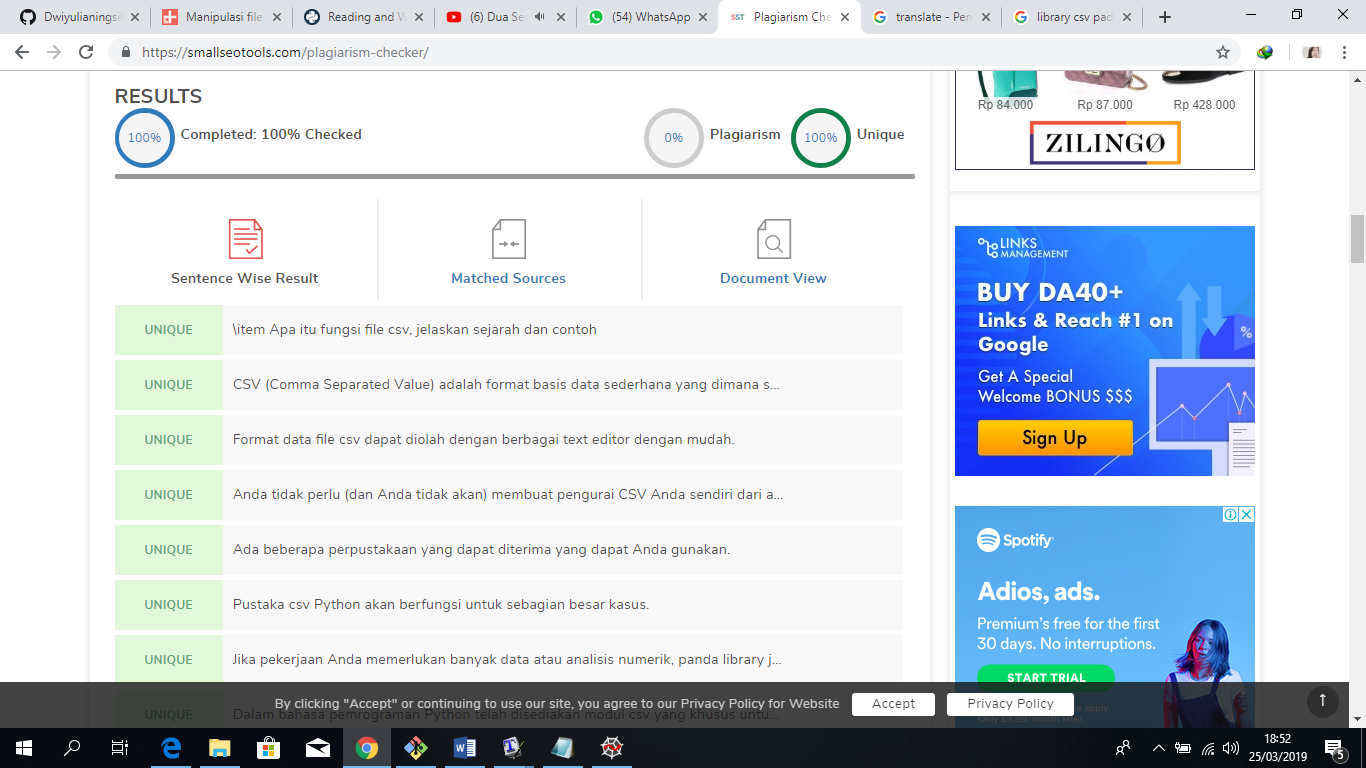
\includegraphics[width=10cm]{figures/4/1174009/yuli.png}
\caption{SS Bebas Plagiarisme}
\label{dwiyul}
\end{figure}


\section{Harun Ar-Rasyid}
\subsection{Soal 1}
File CSV (Nilai Terbatas Koma) adalah jenis file khusus yang dapat Anda buat atau edit di Excel. File CSV menyimpan informasi yang dipisahkan oleh koma, tidak menyimpan informasi dalam kolom. Ketika teks dan angka disimpan dalam file CSV, mudah untuk memindahkannya dari satu program ke program lainnya.
Dari rilis pertama, Excel menggunakan format file biner yang disebut Binary Interchange File Format (BIFF) sebagai format file utamanya. Ini berubah ketika Microsoft merilis Office System 2007 yang memperkenalkan Office Open XML sebagai format file utamanya. Office Open XML adalah file kontainer berbasis XML yang mirip dengan XML Spreadsheets (XMLSS), yang diperkenalkan di Excel 2002. File versi XML tidak bisa menyimpan makro VBA.
Meskipun mendukung format XML baru, Excel 2007 masih mendukung format lama yang masih berbasis BIFF tradisional. Selain itu Microsoft Excel juga mendukung format Comma Separated Values (CSV), DBase File (DBF), SYMbolic LinK (SYLK), Format Interchange Data (DIF) dan banyak format lainnya, termasuk format lembar kerja 1-2 Lotus - 3 (WKS, WK1, WK2, dll.) Dan Quattro Pro.

\subsection{Soal 2}
\begin{itemize}
    \item Texteditor
    Seperti notepad,visual studio code,atom,sublime dan lain sebagainya
    \item Program Spreadsheet
    Seperti excell,google spreadshare,LibreOfficecalc
\end{itemize}

\subsection{Soal 3}
Untuk menulisnya untuk yang paling atas itu kita buat headernya,untuk mepermudah membedakan datanya,dan untuk baris kedua dan seterusnya itu untuk data itu sendiri.
dan setelah di buat kalian save as kemudian pilih format CSV.
dan untuk membukan cukup di double clik file tersebut.

\subsection{Soal 4}
library csv dibuat untuk permudah mengolah data. Dan mempermudah untuk melakukan export dan import file csv itu sendiri

\subsection{Soal 5}
library pandas dibuat agar bahasa pemograman python bisa bersaing R dan matlab, yang digunakan untuk mengolah banyak data , keperluan big data, data mining data science dan sebagainya.

\subsection{Soal 6}
Terdapat 2 fungsi yang bisa digunakan oleh library csv
Pertama,fungsi membaca file csv.
fungsi ini bisa menggunakan list dan dictionary
Dengan list :
\lstinputlisting[firstline=11, lastline=21]{src/4/1174027/teori/c_1174027_csv.py}
Dengan dictionary :
\lstinputlisting[firstline=24, lastline=33]{src/4/1174027/teori/c_1174027_csv.py}
Kedua,fungsi menulis file csv.
\lstinputlisting[firstline=36, lastline=40]{src/4/1174027/teori/c_1174027_csv.py}

\subsection{Soal 7}
Hampir sama dengan library csv,tp library pandas penulisannya lebih sederhana dan terlihat lebih rapih dari pada library csv.
\lstinputlisting[firstline=10, lastline=11]{src/4/1174027/praktek/p_1174027_pandas.py}

\subsection{Bukti Bebas Plagiat}
\begin{figure}[H]
    \centering
    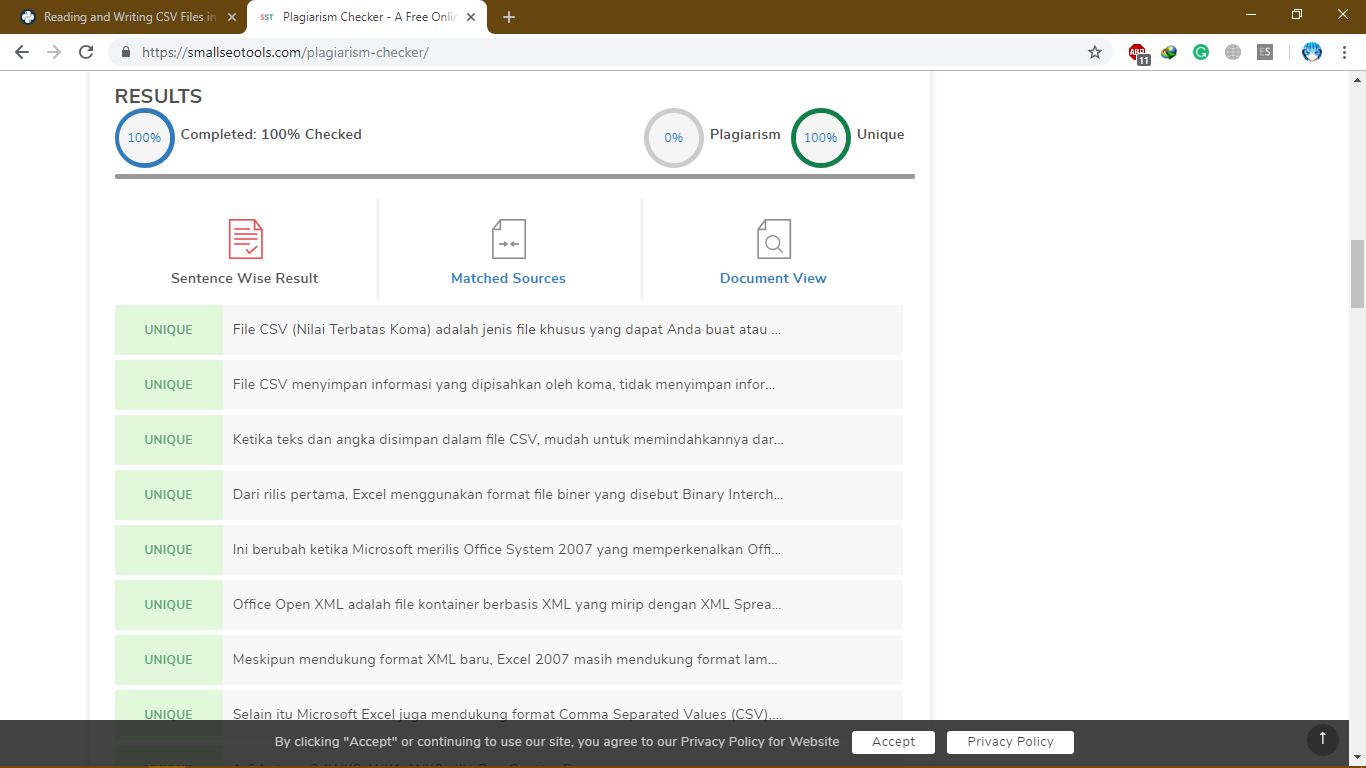
\includegraphics[width=10cm]{figures/4/1174027/teori/harunpla.png}
    \caption{SS Bebas Plagiarisme}
    \label{harun}
\end{figure}

\section{Sri Rahayu}
\subsection{Soal 1}
Isi jawaban soal ke-1

Kalau mau dibikin paragrap \textbf{cukup enter aja}, tidak usah pakai \verb|par| dsb

%\subsection{Soal 2}
%Isi jawaban soal ke-2

%\subsection{Soal 3}
%Isi jawaban soal ke-3

\section{Doli Jonviter}
\subsection{Soal 1}
Isi jawaban soal ke-1

Kalau mau dibikin paragrap \textbf{cukup enter aja}, tidak usah pakai \verb|par| dsb

%\subsection{Soal 2}
%Isi jawaban soal ke-2

%\subsection{Soal 3}
%Isi jawaban soal ke-3

\section{Rahmatul Ridha}
\subsection{Soal 1}
Isi jawaban soal ke-1

Kalau mau dibikin paragrap \textbf{cukup enter aja}, tidak usah pakai \verb|par| dsb

%\subsection{Soal 2}
%Isi jawaban soal ke-2

%\subsection{Soal 3}
%Isi jawaban soal ke-3

\section{Tomy Prawoto}
\subsection{Soal 1}
Isi jawaban soal ke-1

Kalau mau dibikin paragrap \textbf{cukup enter aja}, tidak usah pakai \verb|par| dsb

%\subsection{Soal 2}
%Isi jawaban soal ke-2

%\subsection{Soal 3}
%Isi jawaban soal ke-3

%PRAKTEK
%\chapter{Praktek Library CSV dan Pandas}
%\section{Arjun Yuda Firwanda}
\subsection{Soal 1}
Buatlah fungsi (file terpisah/library dengan nama NPM csv.py) untuk membuka file csv dengan lib csv mode list
\lstinputlisting[firstline=8, lastline=21]{src/4/1174008/praktek/a1174008_csv.py}

\subsection{Soal 2}
Buatlah fungsi (file terpisah/library dengan nama NPM csv.py) untuk membuka file csv dengan lib csv mode dictionary
\lstinputlisting[firstline=23,lastline=55]{src/4/1174008/praktek/a1174008_csv.py}

\subsection{Soal 3}
Buatlah fungsi (file terpisah/library dengan nama NPM pandas.py) untuk membuka file csv dengan lib pandas mode list
\lstinputlisting[firstline=9,lastline=11]{src/4/1174008/praktek/a1174008_pandas.py}

\subsection{Soal 4}
Buatlah fungsi (file terpisah/library dengan nama NPM pandas.py) untuk membuka file csv dengan lib pandas mode dictionary
\lstinputlisting[firstline=13,lastline=16]{src/4/1174008/praktek/a1174008_pandas.py}

\subsection{Soal 5}
Buat fungsi baru di NPM pandas.py untuk mengubah format tanggal menjadi standar dataframe
\lstinputlisting[firstline=18,lastline=20]{src/4/1174008/praktek/a1174008_pandas.py}

\subsection{Soal 6}
Buat fungsi baru di NPM pandas.py untuk mengubah index kolom
\lstinputlisting[firstline=22,lastline=24]{src/4/1174008/praktek/a1174008_pandas.py}

\subsection{Soal 7}
Buat fungsi baru di NPM pandas.py untuk mengubah atribut atau nama kolom
\lstinputlisting[firstline=26,lastline=42]{src/4/1174008/praktek/a1174008_pandas.py}

\subsection{Soal 8}
Buat program main.py yang menggunakan library NPM csv.py yang membuat dan membaca file csv
\lstinputlisting[firstline=8,lastline=10]{src/4/1174008/praktek/main_arjun.py}

\subsection{Soal 9}
Buat program main2.py yang menggunakan library NPM pandas.py yang membuat dan membaca file csv
\lstinputlisting[firstline=12,lastline=14]{src/4/1174008/praktek/main_arjun.py}

\subsection{Penanganan Error}
Dalam praktek kali ini belum menemukan error

\section{Dwi Yulianingsih}
\subsection{Soal 1}
Buatlah fungsi (file terpisah/library dengan nama NPM csv.py) untuk membuka file csv dengan lib csv mode list
\lstinputlisting[firstline=10, lastline=20]{src/4/1174009/praktek/d1174009_csv.py}


\subsection{Soal 2}
Buatlah fungsi (file terpisah/library dengan nama NPM csv.py) untuk membuka file csv dengan lib csv mode dictionary
\lstinputlisting[firstline=22,lastline=34]{src/4/1174009/praktek/d1174009_csv.py}

\subsection{Soal 3}
Buatlah fungsi (file terpisah/library dengan nama NPM pandas.py) untuk membuka file csv dengan lib pandas mode list
\lstinputlisting[firstline=7,lastline=10]{src/4/1174009/praktek/d1174009_pandas.py}

\subsection{Soal 4}
Buatlah fungsi (file terpisah/library dengan nama NPM pandas.py) untuk membuka file csv dengan lib pandas mode dictionary
\lstinputlisting[firstline=12,lastline=15]{src/4/1174009/praktek/d1174009_pandas.py}

\subsection{Soal 5}
Buat fungsi baru di NPM pandas.py untuk mengubah format tanggal menjadi standar dataframe
\lstinputlisting[firstline=17,lastline=19]{src/4/1174009/praktek/d1174009_pandas.py}

\subsection{Soal 6}
Buat fungsi baru di NPM pandas.py untuk mengubah index kolom
\lstinputlisting[firstline=21,lastline=23]{src/4/1174009/praktek/d1174009_pandas.py}

\subsection{Soal 7}
Buat fungsi baru di NPM pandas.py untuk mengubah atribut atau nama kolom
\lstinputlisting[firstline=25,lastline=29]{src/4/1174009/praktek/d1174009_pandas.py}

\subsection{Soal 8}
Buat program main.py yang menggunakan library NPM csv.py yang membuat dan membaca file csv
\lstinputlisting[firstline=8,lastline=10]{src/4/1174009/praktek/main_dwi.py}

\subsection{Soal 9}
Buat program main2.py yang menggunakan library NPM pandas.py yang membuat dan membaca file csv
\lstinputlisting[firstline=12,lastline=14]{src/4/1174009/praktek/main_dwi.py}

\subsection{Penanganan eror}
Ada kalanya saat kita baca file, tapi filenya belum ada. Maka biasanya akan terjadi IOerror.
\lstinputlisting[firstline=8,lastline=8]{src/4/1174009/praktek/eror.py}
maka di tangani dengan cara seperti dibawah ini :
\lstinputlisting[firstline=10,lastline=13]{src/4/1174009/praktek/eror.py}
maka akan muncul peringatan seperti dibawah :
\lstinputlisting[firstline=15,lastline=15]{src/4/1174009/praktek/eror.py}



\section{Harun Ar-Rasyid}
\subsection{Soal 1}
Berikut adalah pemanggilan file csv dengan library csv yang menggunakan list
\lstinputlisting[firstline=10, lastline=20]{src/4/1174027/praktek/c_1174027_csv.py}

\subsection{Soal 2}
Berikut adalah pemanggilan file csv dengan library csv yang menggunakan dictionary
\lstinputlisting[firstline=22, lastline=31]{src/4/1174027/praktek/c_1174027_csv.py}

\subsection{Soal 3}
Berikut adalah pemanggilan file csv dengan library pandas yang menggunakan list
\lstinputlisting[firstline=9, lastline=11]{src/4/1174027/praktek/p_1174027_pandas.py}

\subsection{Soal 4}
Berikut adalah pemanggilan file csv dengan library pandas yang menggunakan dictionary
\lstinputlisting[firstline=13, lastline=16]{src/4/1174027/praktek/p_1174027_pandas.py}

\subsection{Soal 5}
Berikut penggunaan untuk merubah standar penulisan tanggal, yang mengikuti standar penulisan dari pandas.
\lstinputlisting[firstline=18, lastline=20]{src/4/1174027/praktek/p_1174027_pandas.py}

\subsection{Soal 6}
Berikut merupakan pergantian index kolom
\lstinputlisting[firstline=22, lastline=24]{src/4/1174027/praktek/p_1174027_pandas.py}

\subsection{Soal 7}
berikut merupakan penggunaan untuk merename atribut yang digunakan, atau merubah nama header 0
\lstinputlisting[firstline=26, lastline=30]{src/4/1174027/praktek/p_1174027_pandas.py}

\subsection{Soal 8}
\lstinputlisting[firstline=8, lastline=10]{src/4/1174027/praktek/main_harun.py}

\subsection{Soal 9}
\lstinputlisting[firstline=11, lastline=14]{src/4/1174027/praktek/main_harun.py}

\subsection{Penanganan Error}
Dalam praktek kali ini alhamdulliha tidak menemukan error

\section{Sri Rahayu}
\subsection{Soal 1}
Isi jawaban soal ke-1

Kalau mau dibikin paragrap \textbf{cukup enter aja}, tidak usah pakai \verb|par| dsb

%\subsection{Soal 2}
%Isi jawaban soal ke-2

%\subsection{Soal 3}
%Isi jawaban soal ke-3

\section{Doli Jonviter}
\subsection{Soal 1}
\begin{enumerate}
\item Berikut adalah pemanggilan file csv dengan library csv yang menggunakan list
\lstinputlisting[firstline=10, lastline=20]{src/4/1154016/Chapter4/c_1154016_csv.py}

\item Berikut adalah pemanggilan file csv dengan library csv yang menggunakan dictionary
\lstinputlisting[firstline=22, lastline=31]{src/4/1154016/Chapter4/c_1154016_csv.py}

\item Berikut adalah pemanggilan file csv dengan library pandas yang menggunakan list
\lstinputlisting[firstline=9, lastline=11]{src/4/1154016/Chapter4/p_1154016_pandas.py}

\item Berikut adalah pemanggilan file csv dengan library pandas yang menggunakan dictionary
\lstinputlisting[firstline=13, lastline=16]{src/4/1154016/Chapter4/p_1154016_pandas.py}

\item Berikut penggunaan untuk merubah standar penulisan tanggal, yang mengikuti standar penulisan dari pandas.
\lstinputlisting[firstline=18, lastline=20]{src/4/1154016/Chapter4/p_1154016_pandas.py}

\item Berikut merupakan pergantian index kolom
\lstinputlisting[firstline=22, lastline=24]{src/4/1154016/Chapter4/p_1154016_pandas.py}

\item berikut merupakan penggunaan untuk merename atribut yang digunakan, atau merubah nama header 0
\lstinputlisting[firstline=26, lastline=30]{src/4/1154016/Chapter4/p_1154016_pandas.py}
\end{enumerate}

\subsection{Soal 8}
\lstinputlisting[firstline=8, lastline=10]{src/4/1154016/Chapter4/jonviter.py}

\subsection{Soal 9}
\lstinputlisting[firstline=11, lastline=14]{src/4/1154016/Chapter4/jonviter.py}


\section{Rahmatul Ridha}
\subsection{Keterampilan Pemrograman}
\begin{enumerate}
	\item Buatlah  fungsi  (file  terpisah/library  dengan  nama  NPMcsv.py)  untuk  membuka file csv dengan lib csv mode list.
	
	\lstinputlisting[caption = Fungsi untuk membuka file CSV dengan lib CSV mode list., firstline=10, lastline=15]{src/4/1144124/Chapter4/1144124csv.py}
	
	\item Buatlah  fungsi  (file  terpisah/library  dengan  nama  NPMcsv.py)  untuk  membuka file csv dengan lib csv mode dictionary.
	
	\lstinputlisting[caption =  Fungsi untuk membuka file CSV dengan lib CSV mode dictionary., firstline=17, lastline=22]{src/4/1144124/Chapter4/1144124csv.py}
	
	\item Buatlah fungsi (file terpisah/library dengan nama NPMpandas.py) untuk membuka file csv dengan lib pandas mode list.
	
	\lstinputlisting[caption =  Fungsi untuk membuka file CSV dengan lib Pandas mode list., firstline=10, lastline=13]{src/4/1144124/Chapter4/1144124pandas.py}
	
	\item Buatlah fungsi (file terpisah/library dengan nama NPMpandas.py) untuk membuka file csv dengan lib pandas mode dictionary.
	
	\lstinputlisting[caption =  Fungsi untuk membuka file CSV dengan lib Pandas mode dictionary., firstline=10, lastline=13]{src/4/1144124/Chapter4/1144124pandas.py}
	
	\item  Buat fungsi baru di NPMpandas.py untuk mengubah format tanggal menjadi standar dataframe.
	
	\lstinputlisting[caption =  Fungsi untuk mengubah format tanggal menjadi standar dataframe., firstline=15, lastline=19]{src/4/1144124/Chapter4/1144124pandas.py}
	
	\item Buat fungsi baru di NPMpandas.py untuk mengubah index kolom.
	
	\lstinputlisting[caption =  Fungsi untuk mengubah index kolom., firstline=21, lastline=24]{src/4/1144124/Chapter4/1144124pandas.py}
	
	\item Buat fungsi baru di NPMpandas.py untuk mengubah atribut atau nama kolom.
	
	\lstinputlisting[caption =  Fungsi untuk mengubah atribut atau nama kolom., firstline=26, lastline=30]{src/4/1144124/Chapter4/1144124pandas.py}
	
	\item Buat program main.py yang menggunakan library NPMcsv.py yang membuat dan membaca file csv.
	
	\lstinputlisting[caption =  Membuat dan mebaca file CSV menggunakan library 1144124pandas., firstline=8, lastline=13]{src/4/1144124/Chapter4/main.py}
	
	\item Buat program main2.py yang menggunakan library NPMpandas.py yang membuat dan membaca file csv.
	
	\lstinputlisting[caption = Membuat dan mmebaca file CSV menggunakan library 1144124pandas., firstline=8, lastline=13]{src/4/1144124/Chapter4/main2.py}	
\end{enumerate}

\subsection{Penanganan eror}
Saat akan membaca file, akan tetapi file yang akan dibaca belum ada. Maka biasanya akan terjadi IOerror.
\lstinputlisting[firstline=8,lastline=8]{src/4/1144124/Chapter4/error.py}
maka penanganannya dengan cara seperti dibawah ini :
\lstinputlisting[firstline=10,lastline=13]{src/4/1144124/Chapter4/error.py}
dan akan muncul peringatan seperti dibawah :
\lstinputlisting[firstline=15,lastline=15]{src/4/1144124/Chapter4/error.py}

\section{Tomy Prawoto}
\subsection{Soal Praktek}
\begin{enumerate}

\item Buatlah fungsi (file terpisah/library dengan nama NPM csv.py) untuk membuka file csv dengan lib csv mode list
%\lstinputlisting[firstline=8, lastline=21]{src/4/1154121/chapter4/1154121_csv.py}

\item Buatlah fungsi (file terpisah/library dengan nama NPM csv.py) untuk membuka file csv dengan lib csv mode dictionary
%\lstinputlisting[firstline=22,lastline=33]{src/4/1154121/chapter4/1154121_csv.py}

\item Buatlah fungsi (file terpisah/library dengan nama NPM pandas.py) untuk membuka file csv dengan lib pandas mode list
%\lstinputlisting[firstline=9,lastline=12]{src/4/1154121/chapter4/1154121_pandas.py}

\item Buatlah fungsi (file terpisah/library dengan nama NPM pandas.py) untuk membuka file csv dengan lib pandas mode dictionary
%\lstinputlisting[firstline=14,lastline=21]{src/4/1154121/chapter4/1154121_pandas.py}

\item Buat fungsi baru di NPM pandas.py untuk mengubah format tanggal menjadi standar dataframe
%\lstinputlisting[firstline=22,lastline=25]{src/4/1154121/chapter4/1154121pandas.py}

\item Buat fungsi baru di NPM pandas.py untuk mengubah index kolom
%\lstinputlisting[firstline=27,lastline=31]{src/4/1154121/chapter4/1154121pandas.py}

\item Buat fungsi baru di NPM pandas.py untuk mengubah atribut atau nama kolom
%\lstinputlisting[firstline=33,lastline=37]{src/4/1154121/chapter4/1154121pandas.py}

\item Buat program main.py yang menggunakan library NPM csv.py yang membuat dan membaca file csv
%\lstinputlisting[firstline=8,lastline=13]{src/4/1154121/chapter4/main.py}

\item Buat program main2.py yang menggunakan library NPM pandas.py yang membuat dan membaca file csv
%\lstinputlisting[firstline=8, lastline=13]{src/4/1154121/chapter4/main2.py}
\end{enumerate}


%TEORI
%\chapter{Komunikasi Perangkat Keras}
%\section{Harun Ar - Rasyid}
\subsection{Apa itu fungsi device manager di windows dan folder /dev di linux}
Fungsi device manager dan folder /dev itu berfungsi untuk mengetahui device apa saja yang telah terinstal di leptop anda serta mengetahui port yang digunakan oleh device tersebut.

\subsection{Jelaskan langkah-langkah instalasi driver dari arduino}
\begin{enumerate}
    \item Cara Auto
    \begin{itemize}
        \item Pertama Hubungkan sistem minimum Arduino Uno ke komputer dengan kabel USB type B(kabel Printer)
        \begin{figure}[H]	
            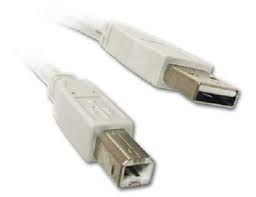
\includegraphics[width=5cm]{figures/5/1174027/teori/1.jpg}
            \centering
            \caption{Membuat file csv}
        \end{figure}

        \item Lalu pada bagian kanan didesktop PC anda, akan muncul popup “Installing device driver software” seperti pada gambar dibawah ini.
        \begin{figure}[H]	
            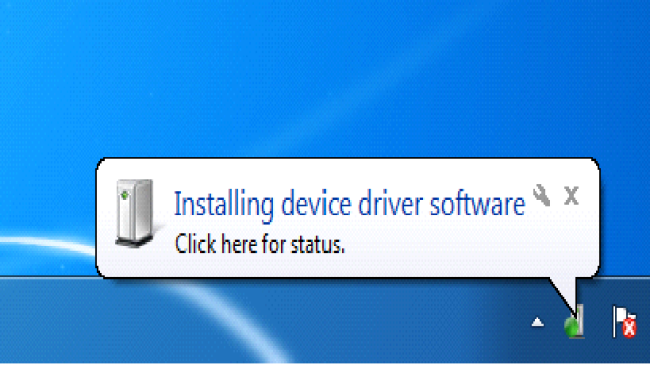
\includegraphics[width=5cm]{figures/5/1174027/teori/2.png}
            \centering
            \caption{Membuat file csv}
        \end{figure}

        \item Tunggu hingga selesai.
        \item Jika sudah selesai anda bisa mengecheck di device manager.
        \begin{figure}[H]	
            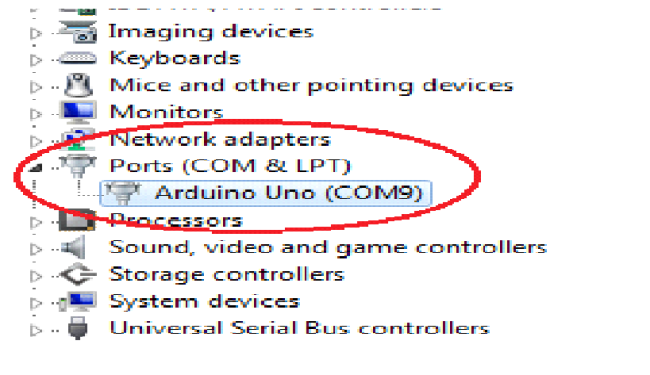
\includegraphics[width=5cm]{figures/5/1174027/teori/11.png}
            \centering
            \caption{Membuat file csv}
        \end{figure}
    \end{itemize}

    \item Cara Manual

    \begin{itemize}
        \item Penginstalan secara manual akan dilakukan jika penginstalan secara auto gagal dilakukan.
        \item Buka Device Manager, caranya pada bagian Search Program and Files lalu ketikkan “device manager”, perhatikan gambar dibawah ini. Pada bagian Control Panel akan muncul Device Manager, klik untuk menjalankan.
            \begin{figure}[H]	
                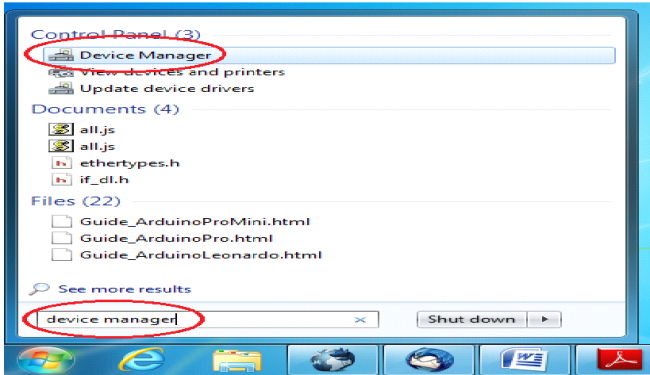
\includegraphics[width=5cm]{figures/5/1174027/teori/4.png}
                \centering
                \caption{Membuat file csv}
            \end{figure}

        \item Cari Unknown device pada bagian Other device, biasanya terdapat tanda seru berwarna kuning, itu disebabkan karena penginstallan tidak berjalan dengan sempurna.
        \begin{figure}[H]	
            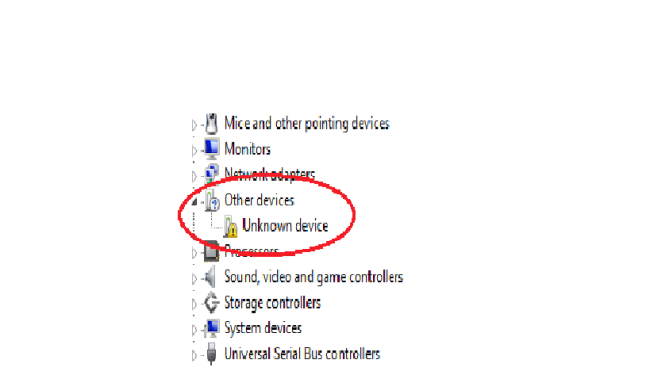
\includegraphics[width=5cm]{figures/5/1174027/teori/5.png}
            \centering
            \caption{Membuat file csv}
        \end{figure}

        \item Klik kanan pada “Unknown device” kemudian pilih Update Driver Software.
        \begin{figure}[H]	
            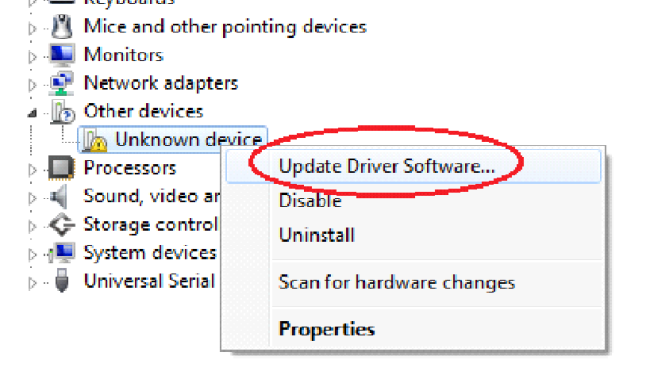
\includegraphics[width=5cm]{figures/5/1174027/teori/6.png}
            \centering
            \caption{Membuat file csv}
        \end{figure}

        \item Pilih Browse my computer for driver software.
        \begin{figure}[H]	
            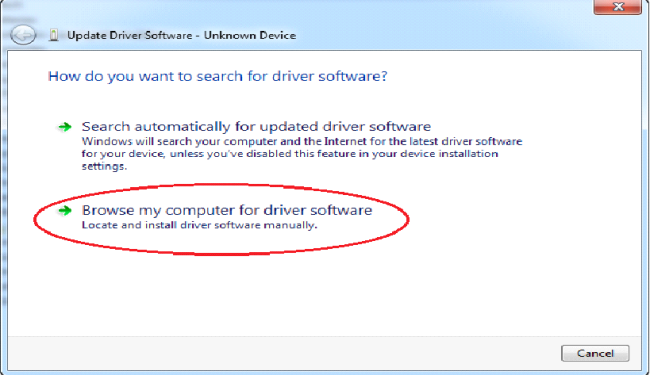
\includegraphics[width=5cm]{figures/5/1174027/teori/7.png}
            \centering
            \caption{Membuat file csv}
        \end{figure}

        \item Arahkan lokasi folder ke folder ..arduino-1.0.5 drivers. Pastikan check-box lalu centang include subfolders. Klik Next untuk melanjutkan instalasi driver.
        \begin{figure}[H]	
            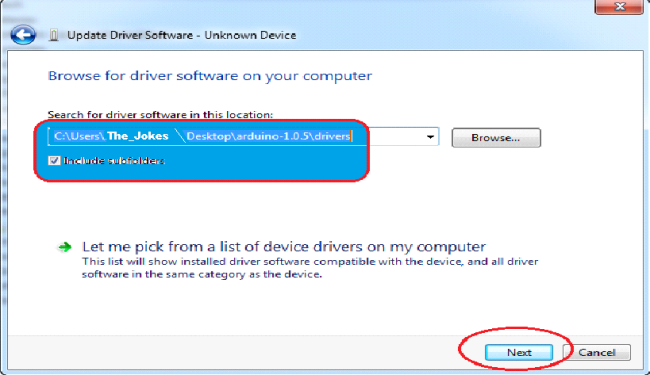
\includegraphics[width=5cm]{figures/5/1174027/teori/8.png}
            \centering
            \caption{Membuat file csv}
        \end{figure}

        \item Kemudian lanjutkan dengan mengklik Install pada tampilan Windows Security.
        \begin{figure}[H]	
            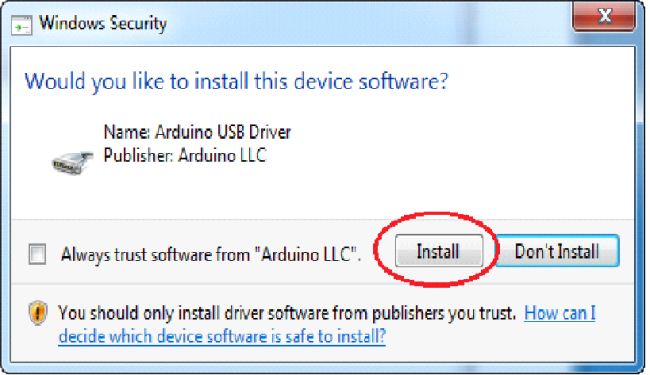
\includegraphics[width=5cm]{figures/5/1174027/teori/9.png}
            \centering
            \caption{Membuat file csv}
        \end{figure}

        \item Jika instalasi driver berhasil maka akan muncul Windows has successfully updated your driver software.
        \begin{figure}[H]	
            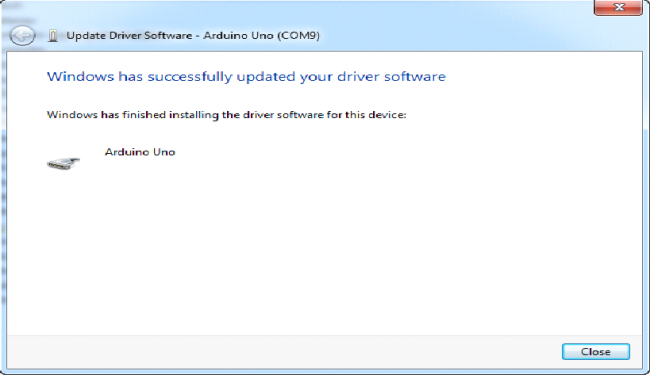
\includegraphics[width=5cm]{figures/5/1174027/teori/10.png}
            \centering
            \caption{Membuat file csv}
        \end{figure}

        \item Perhatikan dan ingat nama COM Arduino Uno, karena nama COM ini yang akan digunakan untuk meng-upload program nantinya.
        \begin{figure}[H]	
            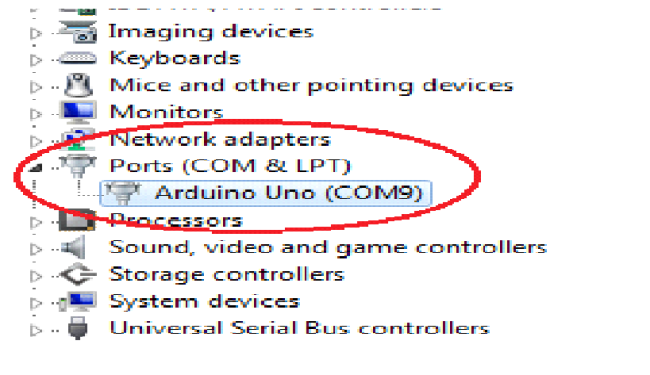
\includegraphics[width=5cm]{figures/5/1174027/teori/11.png}
            \centering
            \caption{Membuat file csv}
        \end{figure}
        \end{itemize}
\end{enumerate}
\subsection{Jelaskan bagaimana cara membaca baudrate dan port dari komputer yang sudah terinstall driver}
Untuk baudrate itu bisa dicek melalui arduino IDE, kemudian untuk mengecheck port bisa dilakukan dengan device manager

\subsection{Jelaskan sejarah library pyserial}
Modul ini merangkum akses untuk port serial. Ini menyediakan backends untuk Python yang berjalan di Windows, Linux, BSD (mungkin sistem yang mendukung POSIX), Jython dan IronPython (.NET dan Mono). Modul bernama "serial" secara otomatis memilih backend yang sesuai. Antarmuka berbasis kelas yang sama pada semua platform yang didukung.
Akses ke pengaturan port melalui properti Python.
Dukungan untuk berbagai ukuran byte, bit stop, paritas dan kontrol aliran dengan RTS / CTS dan / atau Xon / Xoff.
Bekerja dengan atau tanpa menerima batas waktu.
File seperti API dengan "read" dan "write" ("readline" dll. Juga didukung).
File-file dalam paket ini adalah 100 persen Python murni.
Port diatur untuk transmisi biner. Tidak ada stripping byte NULL, terjemahan CR-LF dll. (Yang berkali-kali diaktifkan untuk POSIX.) Ini membuat modul ini bermanfaat secara universal.
Kompatibel dengan pustaka io (Python 2.6+)

\subsection{Jelaskan fungsi-fungsi apa saja yang dipakai dari library pyserial}
Serial – fungsi ini untuk membuka port serial
Write(data) – untuk menulis data lewat port serial
Readline() – untuk membaca string dari port serial
Read(size) – untuk membaca jumlah byte dari port serial
Close() – ini untuk menutup port serial 

\subsection{Jelaskan kenapa butuh perulangan dan tidak butuh perulangan dalam membaca serial}
Perualangan dalam bahasa pemrograman berfungsi menyuruh komputer melakukan sesuatu secara berulang-ulang. Terdapat dua jenis perualangan dalam bahasa pemrograman python, yaitu perulangan dengan for dan while.
Perulangan for disebut counted loop (perulangan yang terhitung), sementara perulangan while disebut uncounted loop (perulangan yang tak terhitung). Perbedaannya adalah perulangan for biasanya digunakan untuk mengulangi kode yang sudah diketahui banyak perulangannya. Sementara while untuk perulangan yang memiliki syarat dan tidak tentu berapa banyak perulangannya.
Perulangan diperlukan agar dapat membaca data secara berulang kali sehingga data yang muncul lebih dari satu.  Sedangkan apabila tidak memakai perulangan maka data akan terbaca satu kali saja.

\subsection{Jelaskan bagaimana cara membuat fungsi yang mengunakan pyserial}
Berikut merupakan contoh penggunaan fungsi yang menggunakan pyserial
\lstinputlisting[firstline=8, lastline=15]{src/5/1174027/teori/T1174027.py}
%PRAKTEK
%\chapter{Komunikasi Perangkat Keras}
%\section{Harun Ar - Rasyid}
\subsection{Soal 1}
\subsection{Soal 2}
\subsection{Soal 3}
\subsection{Soal 4}

%\chapter{Komunikasi Perangkat Keras}
%\section{Rahmatul Ridha}
\subsection{Teori}
\subsubsection{Soal No. 1}
Apa itu fungsi device manager di windows dan folder /dev di linux?

Device manager merupakan perangkat lunak yang berfungsi untuk menampilkan seluruh perangkat keras yang telah di-inisialisasi atau dikenali oleh sistem operasi Windows. Device Manager membantu dalam mengelola atau me-manage semua perangkat keras yang terpasang dan terdeteksi dalam sistem Windows. Perangkat keras tersebut bisa berupa harddisk, kartu VGA, sound, keyboard, perangkat USB dan lain-lainnya.

Fungsi device manager antara lain :
\begin{enumerate}
    \item Mengelola driver perangkat keras.
	\item Menunjukkan informasi detail mengenai suatu perangkat keras.
    \item Mengidentifikasi konflik antar perangkat keras.
	\item Menonaktifkan dan mengaktifkan perangkat keras.
	\item Memberitahukan terjadinya masalah pada perangkat keras.
    \item Menunjukkan status mengenai suatu perangkat keras.
\end{enumerate}

Folder /dev merupakan representasi dari drive yang terhubung sudah ke sistem operasi Linux dan oleh sistem yang dianggap sebagai file-file direktori. Biasanya sering ditampilkan direktori seperti /dev/sdal yang mewakili Drive SATA pertama dalam sistem.

\subsection{Soal No. 2}
Jelaskan langkah-langkah instalasi driver dari arduino!

Berikut ini adalah langkah-langkah instalasi driver dari Arduino UNO di Windows:
\begin{enumerate}
	\item Pertama pastikan Arduino IDE telah terinstall.
	\item Lalu hubungkan port USB Arduino Uno ke port USB PC.
	\item Kemudian PC anda akan mendeteksi perangkat baru yang terpasang dan akan muncul pop seperti \ref{1}.
	\begin{figure}[H]
		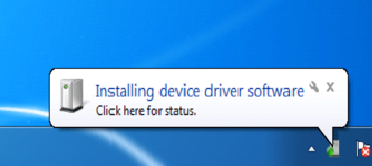
\includegraphics[width=10cm]{figures/5/1144124/Teori/1.png}
		\centering
        \label{1}
	\end{figure}
\item Karena Arduino Uno baru pertama kali terpasang, maka akan muncul pop up error seperti ini.
	\begin{figure}[H]
		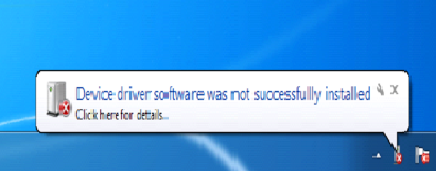
\includegraphics[width=10cm]{figures/5/1144124/Teori/2.png}
		\centering
	\end{figure}
\item Buka `Start' lalu cari Device Manager, kemudian klik `Device Manager'.
	\begin{figure}[H]
		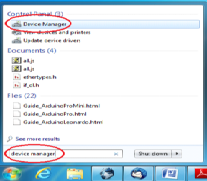
\includegraphics[width=5cm]{figures/5/1144124/Teori/3.png}
		\centering
	\end{figure}
\item Setelah Device Manager terbuka, silahkan cari `Unknown Device' yang berada di Other Device.
	\begin{figure}[H]
		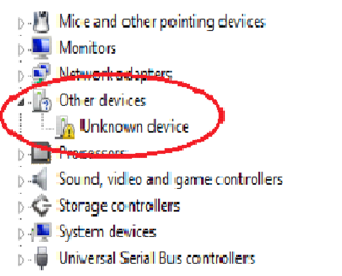
\includegraphics[width=5cm]{figures/5/1144124/Teori/4.png}
		\centering
	\end{figure}
\item Kemudian klik kanan pada `Unknown Device', lalu pilih `Update Driver Software'.
	\begin{figure}[H]
		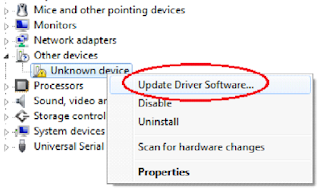
\includegraphics[width=7cm]{figures/5/1144124/Teori/5.png}
		\centering
	\end{figure}
\item Setelah itu muncul window baru, lalu pilih `Browse my computer for driver software'.
	\begin{figure}[H]
		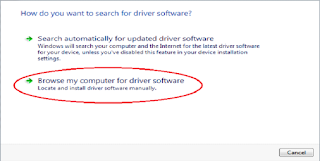
\includegraphics[width=7cm]{figures/5/1144124/Teori/6.png}
		\centering
	\end{figure}
\item Lalu cari folder yang terinstall Arduino IDE dengan mengklik browse. Kemudian klik `Next'.
	\begin{figure}[H]
		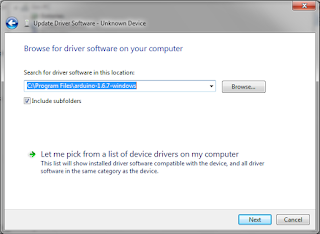
\includegraphics[width=7cm]{figures/5/1144124/Teori/7.png}
		\centering
	\end{figure}
\item Windows akan mencari dan menginstall driver yang berada pada folder tersebut.
	\begin{figure}[H]
		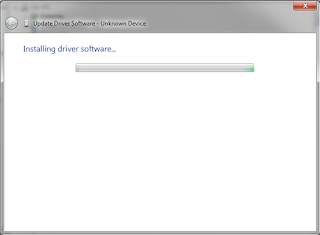
\includegraphics[width=7cm]{figures/5/1144124/Teori/8.png}
		\centering
	\end{figure}
\item Setelah itu akan muncul window, lalu klik `Install'.
	\begin{figure}[H]
		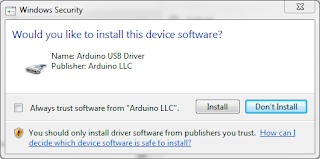
\includegraphics[width=5cm]{figures/5/1144124/Teori/9.png}
		\centering
	\end{figure}
\item Jika berhasil terinstal maka akan muncul window seperti ini.
	\begin{figure}[H]
		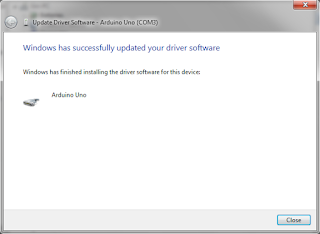
\includegraphics[width=5cm]{figures/5/1144124/Teori/10.png}
		\centering
	\end{figure}
\end{enumerate}

\subsection{Soal No. 3}
Jelaskan bagaimana cara membaca baudrate dan port dari komputer yang sudah terinstall driver!
\textbf{Membaca Baudrate dari Komputer}
\begin{enumerate}
	\item Pertama buka `Start'. Cari `Device Manager', lalu klik.
	\begin{figure}[H]
		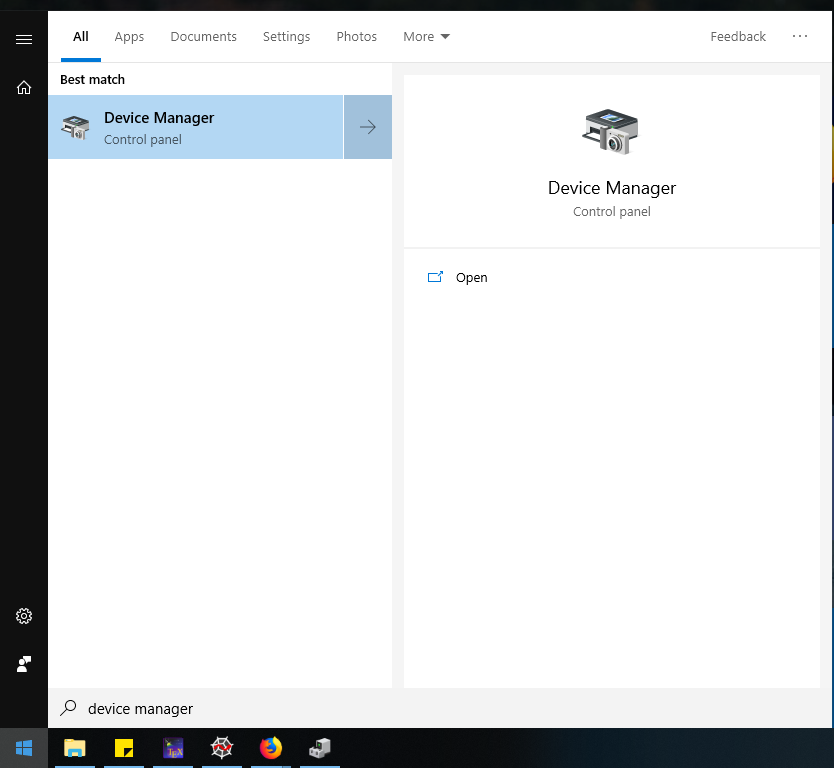
\includegraphics[width=5cm]{figures/5/1144124/Teori/d1.png}
		\centering
	\end{figure}
	\item Kemudian pilih `Ports (COM \& LPT)'.
	\begin{figure}[H]
		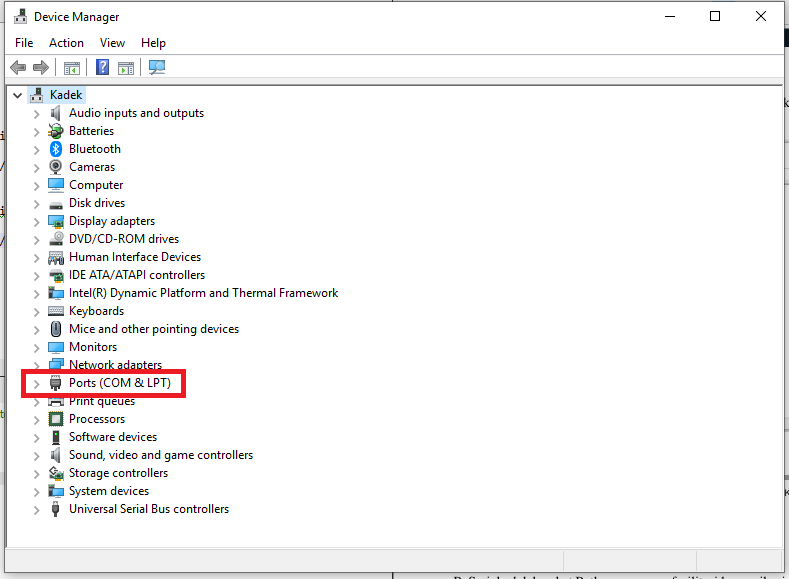
\includegraphics[width=5cm]{figures/5/1144124/Teori/d3.png}
		\centering
	\end{figure}
	\item Klik dua kali pada COM yang terhubung.
	\begin{figure}[H]
		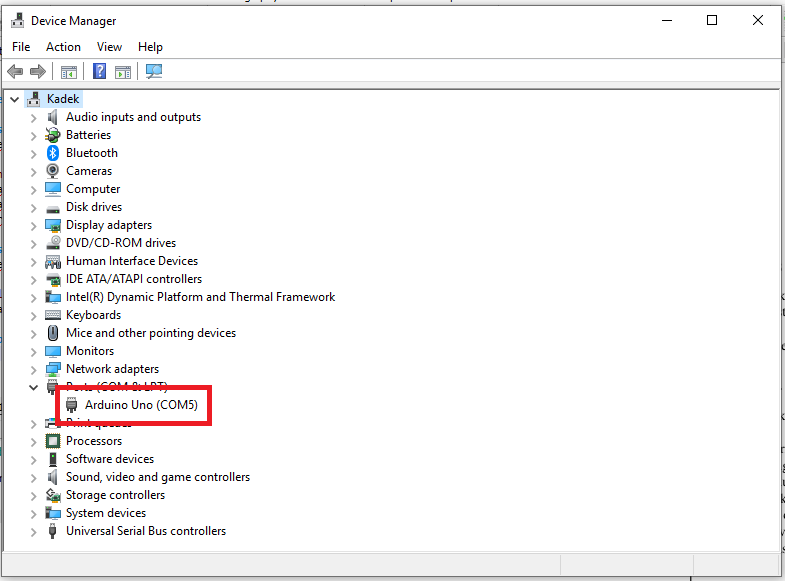
\includegraphics[width=5cm]{figures/5/1144124/Teori/d2.png}
		\centering
	\end{figure}
	\item Pilih tab `Port Settings', lalu lihat di `Bit per second'.
	\begin{figure}[H]
		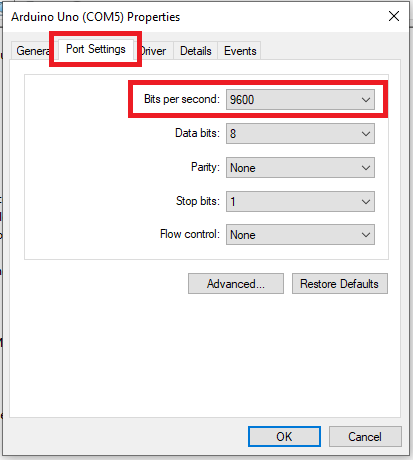
\includegraphics[width=5cm]{figures/5/1144124/Teori/d4.png}
		\centering
	\end{figure}
\end{enumerate}
\textbf{Membaca Port dari Komputer}
\begin{enumerate}
	\item Pertama buka `Start'. Cari `Device Manager', lalu klik.
	\begin{figure}[H]
		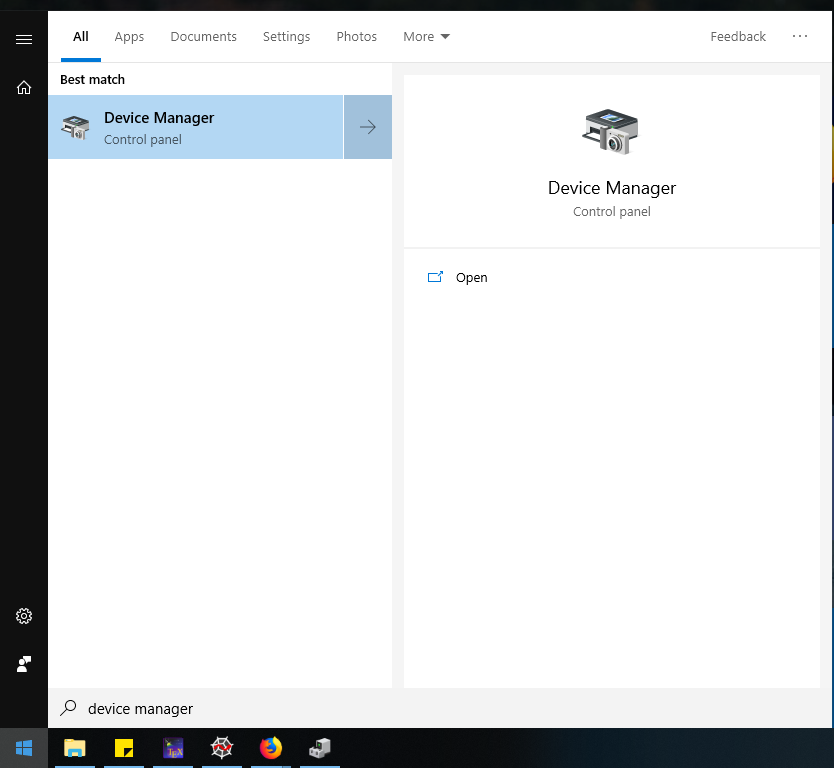
\includegraphics[width=5cm]{figures/5/1144124/Teori/d1.png}
		\centering
	\end{figure}
	\item Kemudian pilih `Ports (COM \& LPT)'.
	\begin{figure}[H]
		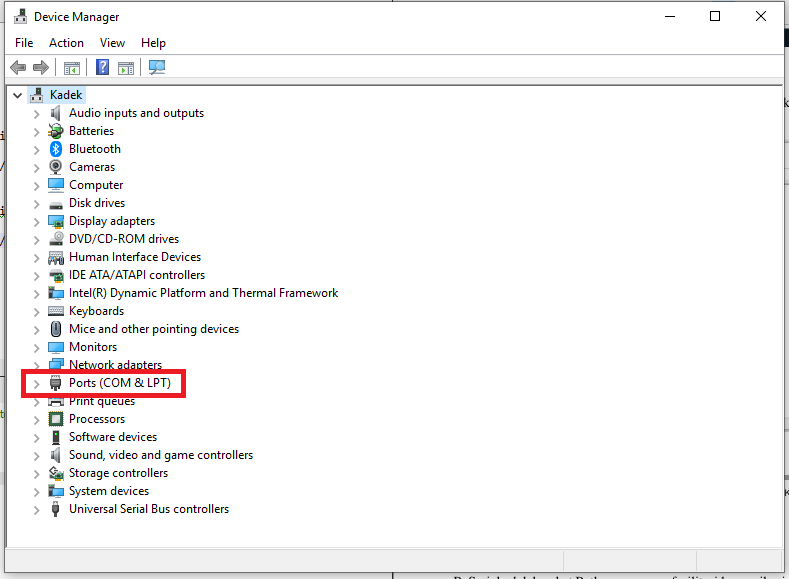
\includegraphics[width=5cm]{figures/5/1144124/Teori/d3.png}
		\centering
	\end{figure}
	\item Port dari Arduino telah terbaca oleh PC.
	\begin{figure}[H]
		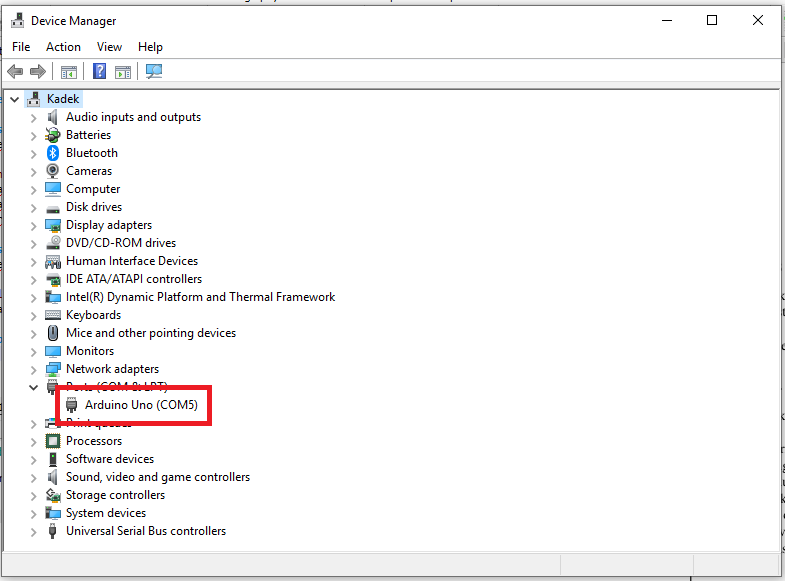
\includegraphics[width=5cm]{figures/5/1144124/Teori/d2.png}
		\centering
	\end{figure}
\end{enumerate}

\subsection{Soal No. 4}
Jelaskan sejarah library pyserial!

PySerial adalah paket Python yang memfasilitasi komunikasi serial antara PC dengan perangkat keras eksternal. PySerial menyediakan antarmuka untuk berkomunikasi melalui protokol komunikasi serial. Komunikasi serial adalah salah satu protokol komunikasi komputer tertua. Protokol komunikasi serial mendahului spesifikasi USB yang dapat digunakan oleh komputer dan perangkat keras lain seperti mouse, keyboard, dan webcam. USB adalah singkatan dari Universal Serial Bus. USB dibangun diatas dan memperluas antarmuka komunikasi serial asli.

\subsection{Soal No. 5}
Jelaskan fungsi-fungsi apa saja yang dipakai dari library pyserial!

Fungsi-fungsi yang dipakai dari library PySerial, yaitu:
\begin{enumerate}
	\item Serial - fungsi ini untuk membuka port serial.
	\item write(data) - fungsi ini menulis data lewat port serial.
	\item readline() - fungsi ini membaca sebuah string dari port serial.
	\item read(size) - fungsi ini untuk membaca jumlah byte dari port serial.
	\item close() - fungsi ini untuk menutup port serial.
\end{enumerate}

\subsection{Soal No. 6}
Jelaskan kenapa butuh perulangan dan tidak butuh perulangan dalam membaca serial!

Pada saat membaca serial di Arduino diperlukan perulangan agar bisa membaca data secara berulang kali sehingga data yang akan muncul banyak. Sedangkan apabila tidak membutuhkan perulangan maka Arduino hanya akan membaca data sekali saja.

\subsection{Soal No. 7}
Jelaskan bagaimana cara membuat fungsi yang mengunakan pyserial!
\lstinputlisting[caption = Fungsi yang menggunakan pyserial., firstline=1, lastline=7]{src/5/1144124/Teori/1144124.py}

\subsection{Praktek}
\subsubsection{Kerjakan soal berikut ini, ....}
\subsubsection{Penanganan Error} 
%\section{Harun Ar - Rasyid}
\subsection{Teori}
\subsubsection{Apa itu fungsi device manager di windows dan folder /dev di linux}
Fungsi device manager dan folder /dev itu berfungsi untuk mengetahui device apa saja yang telah terinstal di leptop anda serta mengetahui port yang digunakan oleh device tersebut.

\subsubsection{Jelaskan langkah-langkah instalasi driver dari arduino}
\begin{enumerate}
    \item Cara Auto
    \begin{itemize}
        \item Pertama Hubungkan sistem minimum Arduino Uno ke komputer dengan kabel USB type B(kabel Printer)
        \begin{figure}[H]	
            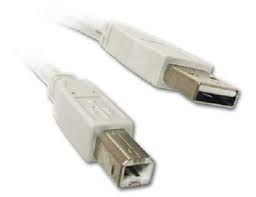
\includegraphics[width=5cm]{figures/5/1174027/teori/1.jpg}
            \centering
            \caption{Membuat file csv}
        \end{figure}

        \item Lalu pada bagian kanan didesktop PC anda, akan muncul popup “Installing device driver software” seperti pada gambar dibawah ini.
        \begin{figure}[H]	
            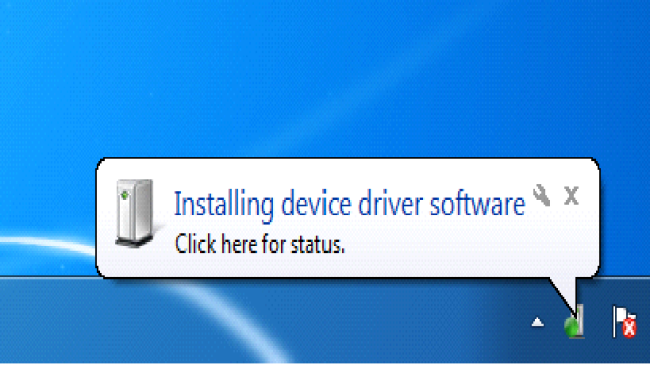
\includegraphics[width=5cm]{figures/5/1174027/teori/2.png}
            \centering
            \caption{Membuat file csv}
        \end{figure}

        \item Tunggu hingga selesai.
        \item Jika sudah selesai anda bisa mengecheck di device manager.
        \begin{figure}[H]	
            \includegraphics[width=5cm]{figures/5/1174027/teori/11.png}
            \centering
            \caption{Membuat file csv}
        \end{figure}
    \end{itemize}

    \item Cara Manual

    \begin{itemize}
        \item Penginstalan secara manual akan dilakukan jika penginstalan secara auto gagal dilakukan.
        \item Buka Device Manager, caranya pada bagian Search Program and Files lalu ketikkan “device manager”, perhatikan gambar dibawah ini. Pada bagian Control Panel akan muncul Device Manager, klik untuk menjalankan.
            \begin{figure}[H]	
                \includegraphics[width=5cm]{figures/5/1174027/teori/4.png}
                \centering
                \caption{Membuat file csv}
            \end{figure}

        \item Cari Unknown device pada bagian Other device, biasanya terdapat tanda seru berwarna kuning, itu disebabkan karena penginstallan tidak berjalan dengan sempurna.
        \begin{figure}[H]	
            \includegraphics[width=5cm]{figures/5/1174027/teori/5.png}
            \centering
            \caption{Membuat file csv}
        \end{figure}

        \item Klik kanan pada “Unknown device” kemudian pilih Update Driver Software.
        \begin{figure}[H]	
            \includegraphics[width=5cm]{figures/5/1174027/teori/6.png}
            \centering
            \caption{Membuat file csv}
        \end{figure}

        \item Pilih Browse my computer for driver software.
        \begin{figure}[H]	
            \includegraphics[width=5cm]{figures/5/1174027/teori/7.png}
            \centering
            \caption{Membuat file csv}
        \end{figure}

        \item Arahkan lokasi folder ke folder ..arduino-1.0.5 drivers. Pastikan check-box lalu centang include subfolders. Klik Next untuk melanjutkan instalasi driver.
        \begin{figure}[H]	
            \includegraphics[width=5cm]{figures/5/1174027/teori/8.png}
            \centering
            \caption{Membuat file csv}
        \end{figure}

        \item Kemudian lanjutkan dengan mengklik Install pada tampilan Windows Security.
        \begin{figure}[H]	
            \includegraphics[width=5cm]{figures/5/1174027/teori/9.png}
            \centering
            \caption{Membuat file csv}
        \end{figure}

        \item Jika instalasi driver berhasil maka akan muncul Windows has successfully updated your driver software.
        \begin{figure}[H]	
            \includegraphics[width=5cm]{figures/5/1174027/teori/10.png}
            \centering
            \caption{Membuat file csv}
        \end{figure}

        \item Perhatikan dan ingat nama COM Arduino Uno, karena nama COM ini yang akan digunakan untuk meng-upload program nantinya.
        \begin{figure}[H]	
            \includegraphics[width=5cm]{figures/5/1174027/teori/11.png}
            \centering
            \caption{Membuat file csv}
        \end{figure}
        \end{itemize}
\end{enumerate}
\subsubsection{Jelaskan bagaimana cara membaca baudrate dan port dari komputer yang sudah terinstall driver}
Untuk baudrate itu bisa dicek melalui arduino IDE, kemudian untuk mengecheck port bisa dilakukan dengan device manager

\subsubsection{Jelaskan sejarah library pyserial}
Modul ini merangkum akses untuk port serial. Ini menyediakan backends untuk Python yang berjalan di Windows, Linux, BSD (mungkin sistem yang mendukung POSIX), Jython dan IronPython (.NET dan Mono). Modul bernama "serial" secara otomatis memilih backend yang sesuai. Antarmuka berbasis kelas yang sama pada semua platform yang didukung.
Akses ke pengaturan port melalui properti Python.
Dukungan untuk berbagai ukuran byte, bit stop, paritas dan kontrol aliran dengan RTS / CTS dan / atau Xon / Xoff.
Bekerja dengan atau tanpa menerima batas waktu.
File seperti API dengan "read" dan "write" ("readline" dll. Juga didukung).
File-file dalam paket ini adalah 100 persen Python murni.
Port diatur untuk transmisi biner. Tidak ada stripping byte NULL, terjemahan CR-LF dll. (Yang berkali-kali diaktifkan untuk POSIX.) Ini membuat modul ini bermanfaat secara universal.
Kompatibel dengan pustaka io (Python 2.6+)

\subsubsection{Jelaskan fungsi-fungsi apa saja yang dipakai dari library pyserial}


Serial – fungsi ini untuk membuka port serial
Write(data) – untuk menulis data lewat port serial
Readline() – untuk membaca string dari port serial
Read(size) – untuk membaca jumlah byte dari port serial
Close() – ini untuk menutup port serial 

\subsubsection{Jelaskan kenapa butuh perulangan dan tidak butuh perulangan dalam membaca serial}


Perualangan dalam bahasa pemrograman berfungsi menyuruh komputer melakukan sesuatu secara berulang-ulang. Terdapat dua jenis perualangan dalam bahasa pemrograman python, yaitu perulangan dengan for dan while.
Perulangan for disebut counted loop (perulangan yang terhitung), sementara perulangan while disebut uncounted loop (perulangan yang tak terhitung). Perbedaannya adalah perulangan for biasanya digunakan untuk mengulangi kode yang sudah diketahui banyak perulangannya. Sementara while untuk perulangan yang memiliki syarat dan tidak tentu berapa banyak perulangannya.
Perulangan diperlukan agar dapat membaca data secara berulang kali sehingga data yang muncul lebih dari satu.  Sedangkan apabila tidak memakai perulangan maka data akan terbaca satu kali saja.

\subsubsection{Jelaskan bagaimana cara membuat fungsi yang mengunakan pyserial}


Berikut merupakan contoh penggunaan fungsi yang menggunakan pyserial
\lstinputlisting[firstline=8, lastline=15]{src/5/1174027/teori/T1174027.py}

\subsubsection{Scan Plagiarisme}
\begin{figure}[H]	
    \includegraphics[width=5cm]{figures/5/1174027/teori/nopla.png}
    \centering
    \caption{Membuat file csv}
\end{figure}

\subsection{Praktek}
\subsubsection{Buatlah fungsi (file terpisah/library dengan nama NPM realtime.py) untuk mendapatkan data langsung dari arduino}
\lstinputlisting[firstline=8, lastline=14]{src/5/1174027/praktek/1174027_realtime.py}

\subsubsection{Buatlah fungsi (file terpisah/library dengan nama NPM save.py) untuk mendapatkan data langsung dari arduino dengan looping}
\lstinputlisting[firstline=8, lastline=15]{src/5/1174027/praktek/1174027_save.py}

\subsubsection{Buatlah fungsi (file terpisah/library dengan nama NPM realtime.py) untuk mendapatkan data dari arduino dan langsung ditulis kedalam file csv}
\lstinputlisting[firstline=16, lastline=29]{src/5/1174027/praktek/1174027_realtime.py}

\subsubsection{Buatlah fungsi (file terpisah/library dengan nama NPM csv.py) untuk membaca file csv hasil arduino dan mengembalikan ke fungsi}
\lstinputlisting[firstline=8, lastline=16]{src/5/1174027/praktek/1174027_csv.py}

\subsubsection{Penanganan Error}
Untuk kali ini saya menemukan Type Error, yaitu error yang menampilkan jika type data na berbeda berusaha disatukan.
\lstinputlisting[firstline=8, lastline=17]{src/5/1174027/praktek/1174027.py}
%\section{Arjun Yuda Firwanda}
\subsection{Teori}
\subsubsection{Apa itu fungsi device manager di windows dan folder /dev di linux}
Fungsi device manager untuk membantu dan mengelola semua hardware yang terpasang dalam suatu windows.

\subsubsection{Jelaskan langkah-langkah instalasi driver dari arduino}
\begin{itemize}
    \item ubungkan sistem minimun Arduino Uno ke komputer dengan kabel USB type B (kabel Printer).
    \item Lalu pada bagian kanan didesktop PC anda, akan muncul popup “Installing device driver software”.
	\item Sistem operasi Windows tidak menyediakan driver untuk Arduino Uno, lalu proses instalasinya harus dilakukan secara manual.
	\item Buka Device Manager, caranya pada bagian Search Program and Files lalu ketikkan “device manager”.
	\item Cari Unknown device pada bagian Other device, terdapat tanda seru yang berwarna kuning, itu disebabkan karena penginstallan tidak berjalan dengan sempurna.
	\item Klik kanan pada “Unknown device”, pilih Update Driver Software.
    \item Pilih Browse my computer for driver software.
	\item Arahkan lokasi folder ke folder arduino-1.0, drivers. Pastikan check-box lalu centang include subfolders. Klik Next untuk melanjutkan instalasi driver.
	\item Kemudian lanjutkan dengan mengklik Install pada tampilan Windows Security.
	\item Jika instalasi driver berhasil maka akan muncul Windows has successfully updated your driver software.
	\item Perhatikan dan ingat nama COM Arduino Uno, karena nama COM ini yang akan digunakan untuk mengupload program nantinya.
\end{itemize}

\subsubsection{Jelaskan bagaimana cara membaca baudrate dan port dari komputer yang sudah terinstall driver}
Untuk baudrate dapat bisa dicek melalui arduino IDE, kemudian untuk mengecek port bisa dilakukan dengan device manager.

\subsubsection{Jelaskan sejarah library pyserial}
Modul ini merangkum akses untuk port serial. Ini menyediakan backends untuk Python yang berjalan di Windows, Linux, BSD (mungkin sistem yang mendukung POSIX), Jython dan IronPython (.NET dan Mono). Modul bernama "serial" secara otomatis memilih backend yang sesuai. Antarmuka berbasis kelas yang sama pada semua platform yang didukung.
Akses ke pengaturan port melalui properti Python. Dukungan untuk berbagai ukuran byte, bit stop, paritas dan kontrol aliran dengan RTS / CTS dan / atau Xon / Xoff. Bekerja dengan atau tanpa menerima batas waktu.
File seperti API dengan "read" dan "write" ("readline" dll. Juga didukung). File-file dalam paket ini adalah 100 persen Python murni. Port diatur untuk transmisi biner. Tidak ada stripping byte NULL, terjemahan CR-LF dll. (Yang berkali-kali diaktifkan untuk POSIX.) Ini membuat modul ini bermanfaat secara universal. Kompatibel dengan pustaka io (Python 2.6+)

\subsubsection{Jelaskan fungsi-fungsi apa saja yang dipakai dari library pyserial}
\begin{itemize}
    \item Serial, fungsi ini untuk membuka port serial
    \item Write(data),  untuk menulis data lewat port serial
    \item Readline, untuk membaca string dari port serial
    \item Read(size), untuk membaca jumlah byte dari port serial
    \item Close, ini untuk menutup port serial 
\end{itemize}

\subsubsection{Jelaskan kenapa butuh perulangan dan tidak butuh perulangan dalam membaca serial}
Perualangan dalam bahasa pemrograman berfungsi untuk menyuruh komputer melakukan sesuatu secara berulang-ulang. Terdapat dua jenis perualangan dalam bahasa pemrograman python diantaranya adalah perulangan dengan for dan while.
Perulangan for atau counted loop (perulangan yang terhitung). Perulangan while atau uncounted loop (perulangan yang tak terhitung). Perbedaannya pada perulangan for biasanya digunakan untuk mengulangi kode yang sudah diketahui banyak perulangannya. Perualangan while untuk perulangan yang memiliki syarat dan tidak tentu berapa banyak perulangannya.
Perualangan digunakan untuk membaca data secara berulang-ulang  dan apabila tidak memakai perulangan, maka data akan terbaca satu per satu.

\subsubsection{Jelaskan bagaimana cara membuat fungsi yang mengunakan pyserial}
\lstinputlisting[firstline=8, lastline=15]{src/5/1174008/teori/T1174008.py}

\subsubsection{Cek Plagiarisme}
\begin{figure}[H]	
    \includegraphics[width=5cm]{figures/5/1174008/teori/ssplagiatchapter5.png}
    \centering
    \caption{Cek Plagiarisme}
\end{figure}

\subsection{Praktek}
\subsubsection{Kerjakan soal berikut ini, ....}
\subsubsection{Penanganan Error}
%\section{Doli Jonviter NT Simbolon /1154016}
{\Large \textbf{Pemahaman Teori}}
\subsection{Soal 1}
Apa itu fungsi device manager di windows dan folder /dev di linux?

\hfill \break
Device Manager  dapat  membantu dalam mengelola  semua hardware yang terpasang  dalam suatu sistem Windows. 
 Berikut fungsi kegunaan Device Manager antara lain adalah :
\begin{enumerate}
	\item Menunjukkan status suatu hardware.
	\item Menunjukkan informasi detil suatu hardware.
	\item Mengelola driver hardware
	\item Disable dan Enable hardware
	\item Mengidentifikasi konflik antar perangkat keras.
\end{enumerate}

\hfill \break
Folder /bin merupakan isi program binner yang harus ada apabila sistem yang dipasang dalam mode single-user, dan juga  ada beberapa program penting seperti bash.

\subsection{Soal 2}
Jelaskan langkah-langkah instalasi driver dari arduino!

\hfill \break
Berikut ini adalah langkah-langkah instalasi driver dari Arduino UNO di Windows:

\begin{enumerate}
	\item Langkah pertama Hubungkan sistem minimun Arduino Uno ke komputer dengan kabel USB .
	\item Lalu pada bagian kanan didesktop PC , akan muncul popup “Installing device driver software” seperti pada gambar dibawah ini.
	\item Kemudian jika sistem  operasi Windows tidak menyediakan driver untuk Arduino Uno,maka harus  melakukan instalasinya harus dilakukan secara manual.
	\item Lalu  Buka Device Manager,  dengan cara pada bagian Search Program and Files lalu ketikkan “device manager” (tanpa tanda petik). 
	\item kemudian Pada bagian COntrol Panel akan muncul Device Manager, lalu klik untuk menjalankan program tersebut.
	\item Setelah itu cari  Unknown device pada bagian Other device, biasanya terdapat tanda seru berwarna kuning, itu disebabkan karena penginstallan gagal.
	\item Klik kanan pada bagian  “Unknown device” kemudian pilih Update Driver Software.
	\item kemudian cari Browse my computer for driver software pada laptop anda.
	\item setelah itu lakukan dengan mengklik Install pada tampilan Windows Security.
	\item Jika instalasi driver pada laptop anda berhasil maka akan muncul Windows has successfully updated your driver software.
	\item Perhatikan dan ingat nama COM Arduino Uno, karena nama COM ini yang akan digunakan untuk meng-upload program nantinya
\end{enumerate}

\subsection{Soal 3}
Jelaskan bagaimana cara membaca baudrate dan port dari komputer yang sudah terinstall driver!
\textbf{Membaca Baudrate dari Komputer}
\begin{enumerate}
	\item Pertama buka `Start'. Cari `Device Manager', lalu klik.
	\begin{figure}[H]
		\includegraphics[width=5cm]{figures/5/1154016/Teori/d1.png}
		\centering
	\end{figure}
	\item Kemudian pilih `Ports (COM \& LPT)'.
	\begin{figure}[H]
		\includegraphics[width=5cm]{figures/5/1154016/Teori/d3.png}
		\centering
	\end{figure}
	\item Klik dua kali pada COM yang terhubung.
	\begin{figure}[H]
		\includegraphics[width=5cm]{figures/5/1154016/Teori/d2.png}
		\centering
	\end{figure}
	\item Pilih tab `Port Settings', lalu lihat di `Bit per second'.
	\begin{figure}[H]
		\includegraphics[width=5cm]{figures/5/1154016/Teori/d4.png}
		\centering
	\end{figure}
\end{enumerate}
\textbf{Membaca Port dari Komputer}
\begin{enumerate}
	\item Pertama buka `Start'. Cari `Device Manager', lalu klik.
	\begin{figure}[H]
		\includegraphics[width=5cm]{figures/5/1154016/Teori/d1.png}
		\centering
	\end{figure}
	\item Kemudian pilih `Ports (COM \& LPT)'.
	\begin{figure}[H]
		\includegraphics[width=5cm]{figures/5/1154016/Teori/d3.png}
		\centering
	\end{figure}
	\item Port dari Arduino telah terbaca oleh PC.
	\begin{figure}[H]
		\includegraphics[width=5cm]{figures/5/1154016/Teori/d2.png}
		\centering
	\end{figure}
\end{enumerate}



\subsection{Soal 4}
Jelaskan sejarah library pyserial!.

\hfill \break
PySerial adalah paket Python yang memfasilitasi komunikasi serial antara PC dengan perangkat keras eksternal. PySerial menyediakan antarmuka untuk berkomunikasi melalui protokol komunikasi serial. Komunikasi serial adalah salah satu protokol komunikasi komputer tertua. Protokol komunikasi serial mendahului spesifikasi USB yang dapat digunakan oleh komputer dan perangkat keras lain seperti mouse, keyboard, dan webcam. USB adalah singkatan dari Universal Serial Bus. USB dibangun diatas dan memperluas antarmuka komunikasi serial asli.

\subsection{Soal 5}
Jelaskan fungsi-fungsi apa saja yang dipakai dari library pyserial!

\hfill \break
Fungsi-fungsi yang dipakai dari library PySerial, yaitu:
\begin{enumerate}
	\item Serial - fungsi ini untuk membuka port serial.
	\item write(data) - fungsi ini menulis data lewat port serial.
	\item readline() - fungsi ini membaca sebuah string dari port serial.
	\item read(size) - fungsi ini untuk membaca jumlah byte dari port serial.
	\item close() - fungsi ini untuk menutup port serial.
\end{enumerate}

\subsection{Soal No. 6}
Jelaskan kenapa butuh perulangan dan tidak butuh perulangan dalam membaca serial!

\hfill \break
Pada saat membaca serial di Arduino diperlukan perulangan agar dapat membaca data secara berulang kali sehingga data yang muncul banyak. Sedangkan apabila tidak membutuhkan perulangan maka Arduino hanya akan membaca data sekali saja.

\subsection{Soal No. 7}
Jelaskan bagaimana cara membuat fungsi yang mengunakan pyserial!

\hfill \break
Fungsi yang berada pada Python, dibuat dengan nama kata kunci def kemudian diikuti dengan nama fungsinya pada pyhton.
Seperti halnya dengan blok kode yang lain, kita juga harus memberikan identasi untuk menuliskan isi fungsi.


\subsection{Praktek}
\subsubsection{Buatlah fungsi (file terpisah/library dengan nama NPM realtime.py) untuk mendapatkan data langsung dari arduino}
\lstinputlisting[firstline=1, lastline=8]{src/5/1154016/1154016_realtime.py}

\subsubsection{Buatlah fungsi (file terpisah/library dengan nama NPM save.py) untuk mendapatkan data langsung dari arduino dengan looping}
\lstinputlisting[firstline=1, lastline=8]{src/5/1154016/1154016_save.py}

\subsubsection{Buatlah fungsi (file terpisah/library dengan nama NPM realtime.py) untuk mendapatkan data dari arduino dan langsung ditulis kedalam file csv}
\lstinputlisting[firstline=9, lastline=18]{src/5/1154016/1154016_realtime.py}

\subsubsection{Buatlah fungsi (file terpisah/library dengan nama NPM csv.py) untuk membaca file csv hasil arduino dan mengembalikan ke fungsi}
\lstinputlisting[firstline=1, lastline=9]{src/5/1154016/1154016_csv.py}

\subsubsection{Penanganan Error}
Untuk kali ini saya menemukan Type Error, yaitu error yang menampilkan jika type data na berbeda berusaha disatukan.
\lstinputlisting[firstline=1, lastline=10]{src/5/1154016/1154016.py}

%\input{chapters/5/1174xxx}
%\input{chapters/5/1174xxx}
%\input{chapters/5/1174xxx}
%\input{chapters/5/1174xxx}

\chapter{matplotlib}
\section{Harun Ar - Rasyid}
\subsection{Teori}
\subsubsection{Apa itu fungsi library matplotlib}
\hfill \break
Matplotlib adalah sebuah library pada python yang digunakan untuk membuat diagram. Library ini biasanya menghasilkan ploting 2D.
\subsubsection{Jelaskan langkah-langkah membuat sumbu X dan Y di matplotlib}
\hfill \break
ntuk membuat sumbu x dan y kita bisa membuatnya menggunakan list untuk mempermudah penyimpanan nilai setiap sumbunya.
Untuk contoh pembuatannya bisa dilihat sebagai berikut
\lstinputlisting[firstline=9, lastline=10]{src/6/1174027/teori/T1174027.py}
\subsubsection{Jelaskan bagaimana perbedaan fungsi dan cara pakai untuk berbagai jenis(bar,histogram,scatter,line dll) jenis plot di matplotlib}
\hfill \break
Untuk perbedaan fungsi plot yang digunakan adalah bentuk bentuk grafik yang akan di tampilkan sesuai dengan perintah yang digunakan pada pemogramannya.
Dan untuk cara pengguna plot tersebut sebagai berikut
\begin{itemize}
    \item line
    Perintah yang digunakan untuk membuat grafik line sebagai berikut.
    \lstinputlisting[firstline=12, lastline=14]{src/6/1174027/teori/T1174027.py}
    \item bar
    Dalam Penggunaan plot bar koordinat x nya itu yang awal, dan untuk Y nya adalah yang kedua
    \lstinputlisting[firstline=16, lastline=25]{src/6/1174027/teori/T1174027.py}
    \item histogram
    Dalam penggunaan plot histogram titik x nya bisa tidak sama dengan titik Y.
    untuk penggunaannya bisa sebagai berikut.
    \lstinputlisting[firstline=27, lastline=34]{src/6/1174027/teori/T1174027.py}
    \item scatter
    Untuk penggunaa plot scatter atau bisa juga d bilang diagram titik.
    Contoh dari penggunaannya bisa dilihat sebagai berikut.
    \lstinputlisting[firstline=36, lastline=49]{src/6/1174027/teori/T1174027.py}
    \item Stack plot
    Untuk penggunaan stack plot ini seperti diagram line, tapi ada fill colornya,jadi antar line itu bisa berdekatan.
    Berikut Contoh penggunaannya
    \lstinputlisting[firstline=82, lastline=92]{src/6/1174027/teori/T1174027.py}
\end{itemize}
\subsubsection{Jelaskan bagaimana cara menggunakan legend dan label serta kaitannya dengan fungsi tersebut}
\hfill \break
Untuk menggunakan legend dan label bisa di lihat dibawah ini
\lstinputlisting[firstline=20, lastline=22]{src/6/1174027/teori/T1174027.py}
penggunaan legend itu untuk mempermudahkita dalam membaca grafik, legend itu sendiri berisi info info dari grafik yang ada seperti nama, kemudian bentuk dan warna.
kemudian untuk label itu sendiri digunakan untuk membedakan nama titik X dan titik Y.
\subsubsection{Jelaskan apa fungsi dari subplot di matplotlib, dan bagaimana cara kerja dari fungsi subplot, sertakan ilustrasi dan gambar sendiri dan apa parameternya jika ingin menggambar plot dengan 9 subplot di dalamnya}
\hfill \break
fungsi dari subplot dari matplotlib untuk bisa membuat lebih dari 1 grafik dalam sebuah program.
untuk cara kerjanya sendiri bisa d cek sebagai berikut
\lstinputlisting[firstline=94, lastline=104]{src/6/1174027/teori/T1174027.py}
untuk parameternya sendiri saya menggunakan x dan y x sebagai koordinat x dan y sebagai koordinat y.
\begin{figure}[H]	
    \includegraphics[width=5cm]{figures/6/1174027/teori/chart.png}
    \centering
    \caption{SubPlot}
\end{figure}
\subsubsection{Sebutkan semua parameter color yang bisa digunakan (contoh: m,c,r,k,... dkk)}
\hfill \break
Untuk parameter color yang bisa digunakan terdiri dari 2 type warna.
\begin{enumerate}
    \item Tipe Warna RGB
    Untuk keterangannya sebagai berikut
    R untuk warna Red atau Merah
    G untuk warna Green atau Hijau
    B untuk warna Blue atau Biru
    \item Tipe warna CMYK
    Untuk keterangannya sebagai berikut
    C untuk warna Cyan atau Biru Muda
    M untuk warna Mangenta atau Merah Tua
    Y untuk warna Yellow Atau Kuning
    K untuk warna blacK atau Hitam
\end{enumerate}
\subsubsection{Jelaskan bagaimana cara kerja dari fungsi hist, sertakan ilustrasi dan gambar sendiri}
\hfill \break
Untuk fungsi histogram ini kedua titik koordinat boleh tidak sama. Misalnya x nya ada 10 nilai sedangkan Y nya ada 5 nilai, itu tidak akan jadi masalah karena diagram ini digunakan untuk mendata usia dari rentang tertentu atau kebutuhan lainnya.
Ini merupakan contoh dari penggunaan histogram
\lstinputlisting[firstline=27, lastline=34]{src/6/1174027/teori/T1174027.py}
dan ini merupakan grafik histogram tersebut.
\begin{figure}[H]	
    \includegraphics[width=5cm]{figures/6/1174027/teori/histogram.png}
    \centering
    \caption{Diagram Histogram}
\end{figure}
\subsubsection{Jelaskan lebih mendalam tentang parameter dari fungsi pie diantaranya labels, colors, startangle, shadow, explode, autopct}
\hfill \break
Berikut penjelasan tentang parameter yang ada dalam pie chart
\begin{itemize}
    \item label
    Label digunakan untuk mempermudah pembaca dalam membaca diagram pie
    \item color
    warna digunakan untuk membedakan antar data
    \item startangle
    Digunakan untuk sudut yang digunakan untuk memulai diagram pie tersebut
    \item shadow
    bayangan digunakan untuk membuat bayangan dari setiap diagram pie yang menonjol
    \item explode
    explode digunakan untuk mengeluarkan suatu data agar data tersebut terlihat menonjol
    \item autopct
    Digunakan sesuai dengan berapa angka dibelakang koma yang kita inginkan
\end{itemize}
\subsection{Praktek}
\subsubsection{Tugas No 1}
\hfill \break
Dibawah ini merupakan penggunaan subplot dan plot bar
\lstinputlisting[firstline=8, lastline=28]{src/6/1174027/praktek/p1174027_bar.py}
Dan dibawah ini merupakan cara pemangilannya
\lstinputlisting[firstline=8, lastline=8]{src/6/1174027/praktek/main_harun.py}
\lstinputlisting[firstline=13, lastline=13]{src/6/1174027/praktek/main_harun.py}

\subsubsection{Tugas No 2}

\hfill \break

Dibawah ini merupakan penggunaan subplot dan plot scatter
\lstinputlisting[firstline=8, lastline=28]{src/6/1174027/praktek/p1174027_scatter.py}
Dan dibawah ini merupakan cara pemangilannya
\lstinputlisting[firstline=9, lastline=9]{src/6/1174027/praktek/main_harun.py}
\lstinputlisting[firstline=14, lastline=14]{src/6/1174027/praktek/main_harun.py}

\subsubsection{Tugas No 3}

\hfill \break

Dibawah ini merupakan penggunaan subplot dan plot pie
\lstinputlisting[firstline=8, lastline=50]{src/6/1174027/praktek/p1174027_pie.py}
Dan dibawah ini merupakan cara pemangilannya
\lstinputlisting[firstline=10, lastline=10]{src/6/1174027/praktek/main_harun.py}
\lstinputlisting[firstline=15, lastline=15]{src/6/1174027/praktek/main_harun.py}

\subsubsection{Tugas No 4}

\hfill \break

Dibawah ini merupakan penggunaan subplot dan plot bar
\lstinputlisting[firstline=8, lastline=28]{src/6/1174027/praktek/p1174027_plot.py}
Dan dibawah ini merupakan cara pemangilannya
\lstinputlisting[firstline=11, lastline=11]{src/6/1174027/praktek/main_harun.py}
\lstinputlisting[firstline=16, lastline=16]{src/6/1174027/praktek/main_harun.py}

\subsection{Penanggan Error}

\hfill \break

Berikut ini merupakan cara penangganan errornya
\lstinputlisting[firstline=8, lastline=14]{src/6/1174027/praktek/1174027.py}
\section{Dwi Yulianingsih}
\subsection{Teori}
\subsubsection{soal 1}
Matplotlib adalah librari plotting 2D Python yang menghasilkan gambar  publikasi bermutu di dalam berbagai format hardcopy dan lingkungan interaktif sepanjang platform. matplotlib dapat digunakan di dalam script Python, shell Python dan ipython), server aplikasi web, dan enam GUI toolkit. matplotlib mencoba untuk membuat hal mudah menjadi lebih mudah dan hal sulit menjadi mungkin. Kamu dapat membuat plot, histogram, power spectra, grafik batang, grafik error, scatterplot, dll, hanya dengan beberapa baris code.

\subsubsection{soal 2}
Pada Matplotlib untuk membuat sumbu X dan Y dapat dilakukan dengan cara yaitu :
\lstinputlisting[firstline=12, lastline=13]{src/6/1174009/chapter6.py}

\subsubsection{soal 3}
\begin{itemize}
\item Sebuah plot sebaran/titik adalah sebuah grafik yang menunjukkan hubungan antara dua set data.
\lstinputlisting[firstline=20, lastline=24]{src/6/1174009/chapter6.py}
\begin{figure}[H]
\centering
\includegraphics[width=7cm]{figures/6/1174009/1b.png}
\caption{Plot sebaran}
\label{dwiyul}
\end{figure}

\item Sebuah histogram adalah grafik yang menampilkan frekuensi data menggunakan batang, dimana angka dikelompokkan dalam rentang tertentu. Dengan kata lain, frekuensi setiap elemen data di dalam daftar ditunjukkan menggunakan histogram. Angka yang dikelompokkan dalam bentuk rentang tertentu disebut bins.
\lstinputlisting[firstline=27, lastline=31]{src/6/1174009/chapter6.py}
\begin{figure}[H]
\centering
\includegraphics[width=7cm]{figures/6/1174009/1c.png}
\caption{Histogram}
\label{dwiyul}
\end{figure}

\item Menggambar sebuah plot garis menggunakan matplotlib. Dalam kasus ini, kita akan menggunakan matplotlib.pyplot, yang menyediakan sebuah framework plotting seperti MATLAB. Dengan kata lain, itu menyediakan sebuah koleksi function bergaya command yang membuat matplotlib berkerja seperti MATLAB.
\lstinputlisting[firstline=12, lastline=17]{src/6/1174009/chapter6.py}
\begin{figure}[H]
\centering
\includegraphics[width=7cm]{figures/6/1174009/1a.png}
\caption{plot garis}
\label{dwiyul}
\end{figure}

\item pie chart adalah diagram yang digunakan untuk membandingkan antar bagian terhadap total. biasanya pie chart dalam bentuk persentase karena nilainya merupakan bagian-bagian yang dijumlah menjadi satu. sehingga bisa lihat kontribusi paling besar atau paling kecil dalam membentuk nilai. Pie chart digunakan untuk perbandingan yang sedikit. pie chart digunakan untuk membandingkan antar bagian terhadap total.
\lstinputlisting[firstline=34, lastline=55]{src/6/1174009/chapter6.py}
\begin{figure}[H]
\centering
\includegraphics[width=7cm]{figures/6/1174009/1d.png}
\caption{pie chart}
\label{dwiyul}
\end{figure}

\item Bagan area benar-benar mirip dengan bagan garis, kecuali area antara sumbu x dan garis diisi dengan warna atau bayangan. Ini mewakili evolusi variabel numerik mengikuti variabel numerik lainnya. Jika kamu ingin mewakili evolusi ini untuk beberapa grup dalam waktu yang bersamaan, Anda mungkin tertarik dengan bagan area bertumpuk, di mana setiap grup ditampilkan satu sama lain.
\lstinputlisting[firstline=58, lastline=77]{src/6/1174009/chapter6.py}
\begin{figure}[H]
\centering
\includegraphics[width=7cm]{figures/6/1174009/1e.png}
\caption{bagan area}
\label{dwiyul}
\end{figure}

\end{itemize}

\subsubsection{soal 4}
Legenda adalah penjelasan garis dilengkapi dengan sampel garis yang dijelaskan. Untuk membuat legenda pada plot anda dapat menggunakan syntax fungsi legend yang dapat dituliskan sebagai berikut:
\lstinputlisting[firstline=76, lastline=76]{src/6/1174009/chapter6.py}
\begin{figure}[H]
\centering
\includegraphics[width=4cm]{figures/6/1174009/legenda.png}
\caption{legenda}
\label{dwiyul}
\end{figure}

Untuk menambah label pada garis sumbu pada grafik dapat menggunakan syntax fungsi xlabel dan fungsi ylabel pada MATLAB. Kedua label ditulis setelah syntax deklarasi plot.
\lstinputlisting[firstline=47, lastline=47]{src/6/1174009/chapter6.py}
\begin{figure}[H]
\centering
\includegraphics[width=4cm]{figures/6/1174009/label.png}
\caption{label}
\label{dwiyul}
\end{figure}


\subsubsection{soal 5}
Ketika fungsi plot dieksekusi, grafik akan ditampilkan dalam figure yang sedang aktif. Untuk beberapa kasus, perlu menampilkan plot grafik dalam figure (multiple figure) yang berbeda ataupun menampilkan lebih dari satu plot dalam satu figure. Hal ini dapat dilakukan dengan menggabungkan plot grafik dalam satu figure.
\lstinputlisting[firstline=80, lastline=80]{src/6/1174009/chapter6.py}
\begin{figure}[H]
\centering
\includegraphics[width=7cm]{figures/6/1174009/multipel.png}
\caption{Histogram}
\label{dwiyul}
\end{figure}


\subsubsection{soal 6}
Kode warna yang digunakan dalam python adalah sebagai berikut:
R adalah warna Merah
G adalah warna Hijau
B adalah warna Biru
M adalah warna Ungu
Y adalah warna Kuning
C adalah warna Biru Muda
K adalah warna Hitam

\subsubsection{soal 7}
pada fungsi histogram titik koordinat tidak boleh sama karena dalam diagram ini digunakan untuk mendata selisih dari hasil rentang nilai tertentu.

\begin{figure}[H]
\centering
\includegraphics[width=7cm]{figures/6/1174009/1c.png}
\caption{Histogram}
\label{dwiyul}
\end{figure}


\subsubsection{soal 8}
\begin{itemize}
\item labels digunakan untuk memberi label/penjelasan dari bagian pie chart yang kita buat.
\item colors digunakan untuk mewarnai pie chart diagram yang telah dibuat, membuat warna yang berbeda antar bagian.
\item startangle digunakan untuk membuat diagram/chart mem-flip atau berbalik arah.
\item explode digunakan untuk menonjolkan salah satu bagian dari pie chart.
\item shadows digunakan untuk memberi bayangan pada pie chart yang kita buat.
\item autopct digunakan untuk memberi persen dari bagian-bagian pie chart yang kita buat.
\end{itemize}

\subsection{Bebas Plagiarisme}
\begin{figure}[H]
\centering
\includegraphics[width=7cm]{figures/6/1174009/plagiaris.png}
\caption{Screenshoot bebas plagiarisme mantap}
\label{dwiyul}
\end{figure}





\section{Arjun Yuda Firwanda}
\subsection{Teori}
\subsubsection{Apa itu fungsi library matplotlib}
\hfill \break
Matplotlib pada python merupakan sebuah library plotting python yang menghasilkan sebuah gambar.

\subsubsection{Jelaskan langkah-langkah membuat sumbu X dan Y di matplotlib}
\hfill \break
Berikut contoh membuat sumbu x dan y yang menggunakan list untuk mempermudah penyimpanan nilai setiap sumbunya adalah sebagai berikut.
\lstinputlisting[firstline=9, lastline=10]{src/6/1174008/teori/T1174008.py}

\subsubsection{Jelaskan bagaimana perbedaan fungsi dan cara pakai untuk berbagai jenis plot di matplotlib}
\hfill \break
Perbedaan fungsi dari segi bentuk grafik pada hasil kode programnya.
Contoh cara pengguna plot tersebut sebagai berikut.
\begin{itemize}
    \item Line
    Plot Line menggunakan perintah untuk membuat grafik line atau garis sebagai berikut.
    \lstinputlisting[firstline=12, lastline=14]{src/6/1174008/teori/T1174008.py}

    \item Bar
    Plot Bar yang memiliki koordinat x dan koordinat y. Berikut contohnya.
    \lstinputlisting[firstline=16, lastline=25]{src/6/1174008/teori/T1174008.py}

    \item Histogram
    Plot Histogram akan menampilkan grafik frekuensi data berdasarkan kode program yang dijalankan.
    Berikut adalah contohnya.
    \lstinputlisting[firstline=27, lastline=34]{src/6/1174008/teori/T1174008.py}

    \item Scatter
    Plot Scatter merupakan diagram yang menghasilkan diagram titik.
    Berikut contoh plot scatter.
    \lstinputlisting[firstline=36, lastline=49]{src/6/1174008/teori/T1174008.py}

    \item Stack plot
    Plot Stack Plot digunakan untuk membuat diagram seperti halnya plot line yang membedakannya dari hal warna. Jadi diagram yang dihasilkan terdapat warna.
    Berikut Contoh penggunaannya.
    \lstinputlisting[firstline=82, lastline=92]{src/6/1174008/teori/T1174008.py}
\end{itemize}

\subsubsection{Jelaskan bagaimana cara menggunakan legend dan label serta kaitannya dengan fungsi tersebut}
\hfill \break
Untuk menggunakan legend dan label bisa di lihat dibawah ini
\lstinputlisting[firstline=20, lastline=22]{src/6/1174008/teori/T1174008.py}
Penggunaan legend pada python untuk mempermudah dalam membaca grafik. Legend berisikan info grafik yang ditampilkan meliputi bentuk, nama, warna. Legend juga digunakan untuk membedakan titik x dan titik y.

\subsubsection{Jelaskan apa fungsi dari subplot di matplotlib, dan bagaimana cara kerja dari fungsi subplot, sertakan ilustrasi dan gambar sendiri dan apa parameternya jika ingin menggambar plot dengan 9 subplot di dalamnya}
\hfill \break
Fungsi subplot untuk membuat lebih dari satu grafik dalam suatu program.
Berikut contohnya.
\lstinputlisting[firstline=94, lastline=104]{src/6/1174008/teori/T1174008.py}

\subsubsection{Sebutkan semua parameter color yang bisa digunakan}
\hfill \break
Untuk parameter color yang bisa digunakan terdiri dari 2 type warna.
\begin{enumerate}
    \item Tipe Warna RGB atau Red sebagai merah, Green sebagai hijau, Blue sebagai biru.

    \item Tipe warna CMYK atau Cyan sebagai biru muda, Magenta sebagai merah tua, Yellow sebagai kuning, Black sebagai hitam.
\end{enumerate}

\subsubsection{Jelaskan bagaimana cara kerja dari fungsi hist, sertakan ilustrasi dan gambar sendiri}
\hfill \break
Fungsi plot histogram sebagai titik koordinat x dan titik koordinat y, yang masing-masing titik koordinat tidak boleh sama. Contoh titik x ada 5 nilai dan titik y ada 7 nilai.
Contoh dari penggunaan histogram
\lstinputlisting[firstline=27, lastline=34]{src/6/1174008/teori/T1174008.py}

\subsubsection{Jelaskan lebih mendalam tentang parameter dari fungsi pie diantaranya labels, colors, startangle, shadow, explode, autopct}
\hfill \break
Berikut penjelasan tentang parameter yang ada dalam pie.
\begin{itemize}
    \item Label
    Label digunakan untuk mempermudah pembaca dalam membaca diagram pie.

    \item Color
    Color atay=u warna digunakan untuk membedakan warna antar data grafik frekuensi.

    \item Startangle
    Startangle digunakan untuk sudut memulai diagram pie.

    \item Shadow
    Shadow atau bayangan digunakan untuk membuat bayangan dari setiap diagram pie yang menonjol.

    \item Explode
    Explode digunakan untuk mengeluarkan suatu data agar data tersebut terlihat menonjol.

    \item Autopct
    Autopct digunakan sesuai dengan berapa angka dibelakang koma yang kita inginkan.
\end{itemize}

\subsection{Scan Bebas Plagiarisme}
\begin{figure}[H]
\centering
\includegraphics[width=7cm]{figures/6/1174008/bebasplagiarisme.png}
\caption{Scan Bebas Plagiarisme}
\label{Bebas Plagiarisme}
\end{figure}

\subsection{Praktek}

\bibliographystyle{IEEEtran}
%\def\bibfont{\normalsize}
\bibliography{references}


%%%%%%%%%%%%%%%
%%  The default LaTeX Index
%%  Don't need to add any commands before \begin{document}
\printindex

%%%% Making an index
%%
%% 1. Make index entries, don't leave any spaces so that they
%% will be sorted correctly.
%%
%% \index{term}
%% \index{term!subterm}
%% \index{term!subterm!subsubterm}
%%
%% 2. Run LaTeX several times to produce <filename>.idx
%%
%% 3. On command line, type  makeindx <filename> which
%% will produce <filename>.ind
%%
%% 4. Type \printindex to make the index appear in your book.
%%
%% 5. If you would like to edit <filename>.ind
%% you may do so. See docs.pdf for more information.
%%
%%%%%%%%%%%%%%%%%%%%%%%%%%%%%%

%%%%%%%%%%%%%% Making Multiple Indices %%%%%%%%%%%%%%%%
%% 1.
%% \usepackage{multind}
%% \makeindex{book}
%% \makeindex{authors}
%% \begin{document}
%%
%% 2.
%% % add index terms to your book, ie,
%% \index{book}{A term to go to the topic index}
%% \index{authors}{Put this author in the author index}
%%
%% \index{book}{Cows}
%% \index{book}{Cows!Jersey}
%% \index{book}{Cows!Jersey!Brown}
%%
%% \index{author}{Douglas Adams}
%% \index{author}{Boethius}
%% \index{author}{Mark Twain}
%%
%% 3. On command line type
%% makeindex topic
%% makeindex authors
%%
%% 4.
%% this is a Wiley command to make the indices print:
%% \multiprintindex{book}{Topic index}
%% \multiprintindex{authors}{Author index}

\end{document}

